%##########################################
\section{Broadband Power Transfer Networks}
\label{sec_wurc_pa_design}

%\rgnote{This is a brief of the content that will be presented here--I have models, simulations, and a discussion of the new design approach (and why alternative methods don't work). This is a contribution that first formulates a numerical optimization framework for wideband matching building on Yarman's real frequency techniques, and then solves it to produce a seed mathching circuit design. We show that although Yarman leaves off here, that is not sufficient to realize a practical solution and that additional parasitic models and empirical design techniques must be used to bring the design to realization. I'm cleaning up the plots and code to expand this section right now.}

	In order to operate as an opportunistic transmitter in the UHF band and adapt to various channel bandwidths, spectrum availability, and regulatory domains across the world, \ac{WURC} is designed to operate at arbitrary channel bandwidths from 1.5 - 28~MHz with center frequencies ranging from 470 - 700~MHz on its 75~$\Omega$ UHF antenna ports, and 2400 - 2500~MHz on its 50~$\Omega$ ISM antenna ports. 

	We target a design goal of radio output power up to 30~dBm from 470 to 700~MHz, the maximum conducted power to the antenna currently allowed by the \ac{FCC} in the United States for unlicensed operation within a single 6~MHz UHF channel \cite{flores2013ieee80211af}.\footnote{The 30~dBm limit is measured at the input RF connector to the antenna. \ac{FCC} regulation allows up to 36~dB \ac{EIRP} when including passive antenna gain. With antenna gain greater than 6~dB, the conducted power limit is decreased by 1~dB for each 1~dB of additional antenna gain in order to maintain a 36~dBm \ac{EIRP} maximum per 6~MHz channel. When channels are bonded, the total power budget for all channels is increased according to the total number of bonded channels \cite{fcc2015ro}.}
	The 2.4~GHz ISM transmit chain provides up to 27~dBm between 2400 - 2500~MHz.
	%The wide UHF frequency range presents a challenge for a high-power RF design since power amplifiers and their associated impedance matching networks are generally optimized for a narrow frequency band.

	By targeting nominal operation between 470 - 700~MHz, the \ac{WURC} analog front end utilizes a passband that is approximately $\frac{2\cdot(700-470)}{700+470}\cdot 100\% = 39.3\%$ wide, which is a significant design challenge.
	Intuitively, the wide 160~MHz channels for 802.11ac or 2.16~GHz for 802.11ad standards seem large, but they only represent a percent bandwidth of 3.1\% and 3.6\%, respectively, making their power transfer networks more simple.\footnote{Accurate physical modeling and parasitics are more of a concern at 5.8 and 60~GHz than is achieving a wide bandwidth power transfer match.}
	The efficiency of a \emph{passive} power transfer network will fundamentally trade off with the operational bandwidth of that network, as first proved by Fano for a simple RC capacitive load \cite{fano1950theoretical}.
	Fano's fundamental limit motivates the need to optimize the efficiency of the passive transfer network that delivers power to the various amplification stages of \ac{WURC}.
	As we will show, this process is non-trivial and requires multiple iterations utilizing various design techniques.

	In this section, we will first utilize real frequency techniques to construct an optimization problem and numerically solve for an ideal solution for the passive broadband power transfer network design.
	We will then show that this solution is inadequate to actually realize in a passive lumped element circuit, which will require us to develop empirical models of our circuit elements and layout to accurately capture parasitic circuit elements.
	This will finally allow us to synthesize a physical circuit realization that meets design goals.
	The circuit is manufactured, tested, and validated with consistent results that eventually match simulated results.

%%##################################################
%\subsection{Power Transfer Network Synthesis}
%\label{sec_match_synthesis}
%
%\rgnote{content snipped from paper follows, FIXME} 
%
%
%A common technique for designing high-power analog front-ends is to build multiple switched amplification and filtering chains, each optimized for a narrow band.
%However, when the system operating frequency range spans multiple octaves, space and cost constraints require that each chain support a wide range of frequencies.
%In the design of \ac{WURC}, we target two optimized transmit and receive chains for 470-698~MHz and 2400-2500~MHz, chosen because these two bands allow unlicensed operation and are invaluable for research and testing.
%
%
%
%Since the bandwidth of an RF chain is generally proportional to $\Delta f/f$, common techniques for designing and implementing discrete power transfer networks (e.g., multi-section Chebyshev transformers \cite{grebennikov2005rf}) either cannot meet design requirements for passband flatness or result in non-realizable circuits when applied to bandpass designs spanning a large frequency range like 470-698 MHz.

% ###################################
\subsection{Real Frequency Technique for Initial Circuit Synthesis}
\label{sec_dual_match}

%\rgnote{State the GEL dual matching problem here.}
%
%\begin{figure}[h]
%\centering
  %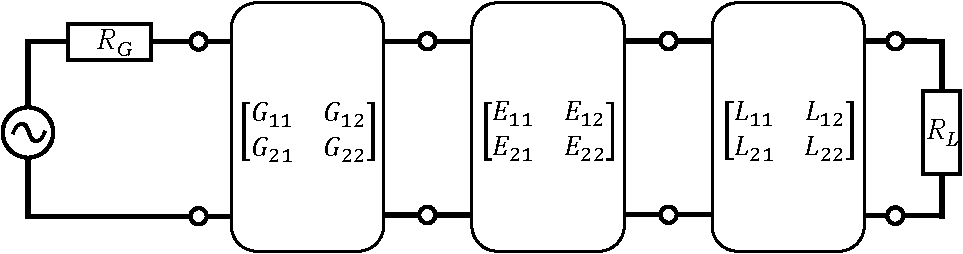
\includegraphics[width=0.67\linewidth]{figs/matching/matching_gel}   
    %\caption{Block diagram of dual matching problem with Darlington source and load representations.}
%\label{fig_matching_gel}
%\end{figure}

 	Several traditional analog design techniques can be used to design a passive matching network for amplifier circuits, such as an analytical conjugate match \cite{orfanidis2002electromagnetic} \S13, the direct design approach using the Smith Chart \cite{grebennikov2005rf} \S3.3, or prototype filter design \cite{grebennikov2005rf} \S10.7.	
	However, in the case that the desired passive matching network must match a complex real-world device over a large bandwidth, then these traditional design techniques become ``inaccessible'' \cite{yarman2010design, chen2015broadband}.
	Specifically, analytical and direct design techniques can yield physically feasible results for narrowband matches but produce negative-valued resistances, require the use of ideal transformers, or require very high-order circuits with a large number of components for wideband matches.
	Unfortunately, while useful for developing circuit theory, each of these outcomes is either not possible or extremely impractical to actually implement with a passive physical circuit.
	
	Instead, we utilize the real frequency matching technique proposed and developed by Carlin and Yarmin \cite{carlin1977new, carlin1983double, yarman1982simplified} which utilizes numerical methods to solve for a piecewise approximation to the reflection coefficient of the optimal matching network.
	The entire set of matching network S-parameters are determined from a series of identities and Belevitch factorizations of the single reflection coefficient \cite{yarman1982simplified}.
	Finally, an LC-ladder circuit can be realized with a simple lumped element passive circuit using long division(\cite{yarman2010design} \S9.7).
	We repeat this optimization for both the input and the output matching network for each amplifier component separately rather than using the cascaded gain stage approach proposed by Yarmin \cite{carlin1983double} for practical reasons: we find that physical circuit layout is improved when each amplifier component is individually matched to the system characteristic impedance rather than to each other, allowing arbitrary placement of the components.

% ######################
\subsubsection{Broadband Matching Problem Statement}
\label{sec_srft_problem_statement}
	
	Our objective is to maximize the \ac{TPG} of our chosen broadband amplifiers across the target band of operation utilizing only passive, lumped-element power transfer, or ``matching'' networks between the source \ac{SDR} transceiver, analog pre-amplifier and power amplifier stages, and the antenna.
	We choose to target a flat frequency response within the 470 - 700~MHz passband, thereby simplifying operation while maximizing the Bode-Fano bandwidth-efficiency tradeoff  \cite{bode1945network, fano1950theoretical}.
	
	The active amplifier circuits for the TQP3M9009 and RFPA3800 are represented by their de-embedded two-port S-parameter representations (Section~\ref{sec_scattering}) obtained from the component vendors and validated using evaluation boards for each component.
	In the case where the component S-parameter data are sampled at different frequency intervals, we observe that their real and imaginary components are individually smooth functions and therefore we can linearly interpolate the real and imaginary components separately with negligible loss in their S-parameter representation accuracy before recombining into a sequence of complex $\mathbf{S}[\omega_i]\in\mathbb{C}^{2\times 2}$ matrices indexed by uniform frequency intervals $\omega_i$.
	The original technique proposed by Carlin \cite{carlin1977new} also solved for the optimal ``break points,'' or arbitrary frequency points for representing the sampled reflection coefficients; however, we simplify the problem formulation by choosing uniform break points and oversampling substantially.
	Modern computational capabilities permit this luxury.
	
	Assuming a steady-state input stimulus and linear operating regime,\footnote{While our small-signal technique does not, in general, optimize the performance of the system when the amplifier becomes saturated, we claim first that energy efficiency was not one of our design goals, therefore operating the amplifier near saturation is not desired; and second, the design paradigm of many-antenna wireless systems is to \emph{reduce} the power budget of any single radio chain while relying on array beamforming gain to provide the link budget necessary for communication. Therefore, we always expect to operate this design in the amplifier's linear operating regime, which is where small-signal techniques excel.} the first stage amplifier system for optimization can be represented as in Figure~\ref{fig_matching_stage_1}.
	
\begin{figure}[h]
\centering
  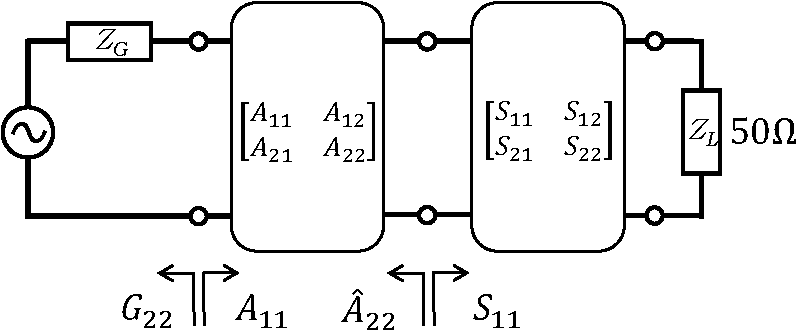
\includegraphics[width=0.67\linewidth]{figs/matching/matching_stage_1}   
    \caption{First stage of the dual matching problem with an active amplifier.}
\label{fig_matching_stage_1}
\end{figure}

	%In the first half of the optimization, we consider the partial system shown in Figure~\ref{fig_matching_stage_1}.
	Both the source impedance, $Z_G(\omega)$, and the amplifier itself, $\mathbf{S}(\omega)$, are parametrized with scattering parameters, allowing the complex frequency response of the amplifier to be represented with empirical data.
	For this stage, the load impedance is set to be purely resistive: $Z_L(\omega) = Z_0 = 50~\Omega$.

% ############### 
\subsubsection{Real Frequency Objective Function Stage 1}
\label{sec_srft_stage_1}

	With this simplification, our goal is to find the input matching network as a function of angular frequency, $\textbf{A}(\omega)$, that maximizes the flat \ac{TPG} of the active amplifier cascaded into a 50-$\Omega$ load, or formally:
	\begin{equation} \label{eq_stage_1}
		\argmax_{[\textbf{A}(\omega)]}{[T_1(\omega) - T_{01}]},
	\end{equation}
where the first stage \ac{TPG} is
	\begin{equation} \label{eq_stage_1_tpg}
		{T_1(\omega)} = |G_{21}|^2\frac{|A_{21}|^2}{|1-A_{11}G_{22}|^2\cdot|1-\hat{A}_{22}S_{11}|^2}|S_{21}|^2,
	\end{equation}
and the target flat \ac{TPG}, $T_{01}$, is set by the engineer.
	A reasonable value for $T_{01}$ can be more systematically determined by setting $T_{01}$ to the minimum value of the amplifier's \ac{MAG} within the band of interest and decreasing $T_{01}$ until an acceptable solution to Equation~\ref{eq_stage_1} is found.
	For an active amplifier in a nominal 50~$\Omega$ circuit, the \ac{MAG} for an unconditionally stable \cite{orfanidis2002electromagnetic} amplifier is defined as 
\begin{equation} \label{eq_mag}
T_{MAG} := \frac{|S_{21}|^2}{(1-|S_{11}|^2)(1-|S_{22}|^2)}.
\end{equation}

	In Equation~\ref{eq_stage_1_tpg}, we let $p:=j\omega$ and the unknown $\mathbf{A}(\omega)$ is completely determined by the polynomial
\begin{equation}	
\hat{A}_{22}(p) = \frac{h(p)}{g(p)} = \frac{h_np^n+\dotsb+h_1p+h_0}{g_np^n+\dotsb+g_1p+g_0}, \label{eq_belevich_poly}
\end{equation}
where the optimization is taken over just the coefficients of $h(p)$, since all other terms can be derived uniquely from $h(p)$ as shown by Yarman \cite{yarman1982simplified}.
	First, the solution matching equalizer is assumed lossless, therefore we restrict solutions to those that obey the lossless criterion $$g(p)g(-p)=h(p)h(-p)+(-1)^k p^{2k} ~>~ 0 ~\forall p,$$
which provides the means to derive $g(p)$ from $h(p)$. %G(p^2)=
	The remaining terms are also derived as:\footnote{There is a typo in \cite{yarman2010design} with incorrect derivation of $A_{11}(p)$. The equations given here are correct and verified with working examples.}
\begin{align}
	A_{12}(p) &= A_{21}(p) = \textpm \frac{p^k}{g(p)} \\
	A_{11}(p) &= -(-1)^k\frac{h(-p)}{g(p)}.
\end{align}

	The number of reactive circuit elements is set implicitly by allocating the initial polynomial solution $h(p)$ with length $n$.
	The order of the zero of the transmission coefficients $A_{12}(p)$ at DC is also set to $k \in \mathbb{Z} \geqslant 0$ by the engineer, thus providing all the remaining unknowns and allowing the optimization to continue.
	In our case, we set $k=0$ in order to avoid additional components needed to produce zeros at DC; this produces a lowpass circuit.
	This could introduce some inefficiency in our synthesized matching circuit since the Bode-Fano limit suggests zeroing gain outside of the desired passband \cite{bode1945network, fano1950theoretical}, however we find that the tradeoff in reducing the number of components to realize the circuit to be worth it.
	
% ############### 
\subsubsection{Real Frequency Objective Function Stage 2}
\label{sec_srft_stage_2}

\begin{figure}[h]
\centering
  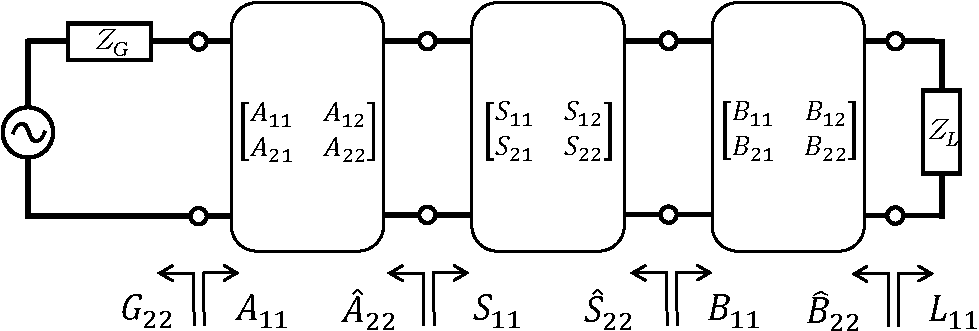
\includegraphics[width=0.8\linewidth]{figs/matching/matching_stage_2}   
    \caption{Second stage of the dual matching problem with an active amplifier.}
\label{fig_matching_stage_2}
\end{figure}

	Once the input matching equalizer has been synthesized, we then change the load impedance from a nominal $50~\Omega$ to $Z_L(\omega)$, which may be a constant scalar value represented by its Darlington 2-port equivalent reflection coefficients \cite{yarman2010design} or may be specified empirically by measured or modeled 2-port S-parameters $\textbf{L}(\omega)$.
	We fix $\textbf{A}(\omega)$ to the optimal value found for Equation~\ref{eq_stage_1} and define a new optimization objective function for the cascaded \ac{TPG} for the system extended in Figure~\ref{fig_matching_stage_2}:
\begin{equation} \label{eq_stage_2}
	\argmax_{[\textbf{B}(\omega)]}{[T_2(\omega) - T_{02}]},
\end{equation}
where the second stage \ac{TPG} is
\begin{equation} \label{eq_stage_2_tpg}
	{T_2(\omega)} = \overbar{T_1}(\omega)\frac{|B_{21}|^2}{|1-B_{11}\hat{S}_{22}|^2\cdot|1-\hat{B}_{22}L_{11}|^2}|L_{21}|^2,
\end{equation}
and $\overbar{T_1}(\omega)$ is the piecewise optimized \ac{TPG} for the numerical solution for Equation~\ref{eq_stage_1} and the system in Figure~\ref{fig_matching_stage_1}.

	In order to solve the two posed optimization problems, we develop a MATLAB script utilizing modified functions from Yarman \cite{yarman2010design} and write an error function taking the numerator from Equation~\ref{eq_belevich_poly} as an argument and outputting the error function from Equations~\ref{eq_stage_1} and \ref{eq_stage_2} for optimization.
	Using MATLAB's non-linear optimization toolbox utilizing the Levenberg-Marquardt least-squares optimization algorithm \cite{hansen2013least}, it is possible to converge on a satisfactory solution.
	Since the optimization is highly sensitive to the initial conditions of the polynomial in Equation~\ref{eq_belevich_poly}, we run the algorithm starting with all combinations of the coefficients of $h(p)$, \{$h_0 + \ldots + h_k\} = \{\pm 1, \ldots , \pm 1 \}$ and choose the result with the smallest error.
	While this would be prohibitive for large-sized problems, we find it works well for problems with 2-10 passive components; any more components and the set of starting conditions would be too large to exhaustively search and the physical circuit implementation would be quite large and sensitive to component tolerance.
	
	Finally, there do not appear to be strict guarantees that the proposed optimization will always converge for all input data sets nor that the global minimum will be found utilizing our starting conditions.
	Nevertheless, we found this optimization to be well-behaved and did not encounter any conditions that resulted in a failure to converge upon a satisfactory solution.
	
	\begin{figure*}[th]
\centering        
   	\subfigure[TQP3M9009 Reflection Coefficients.]{
		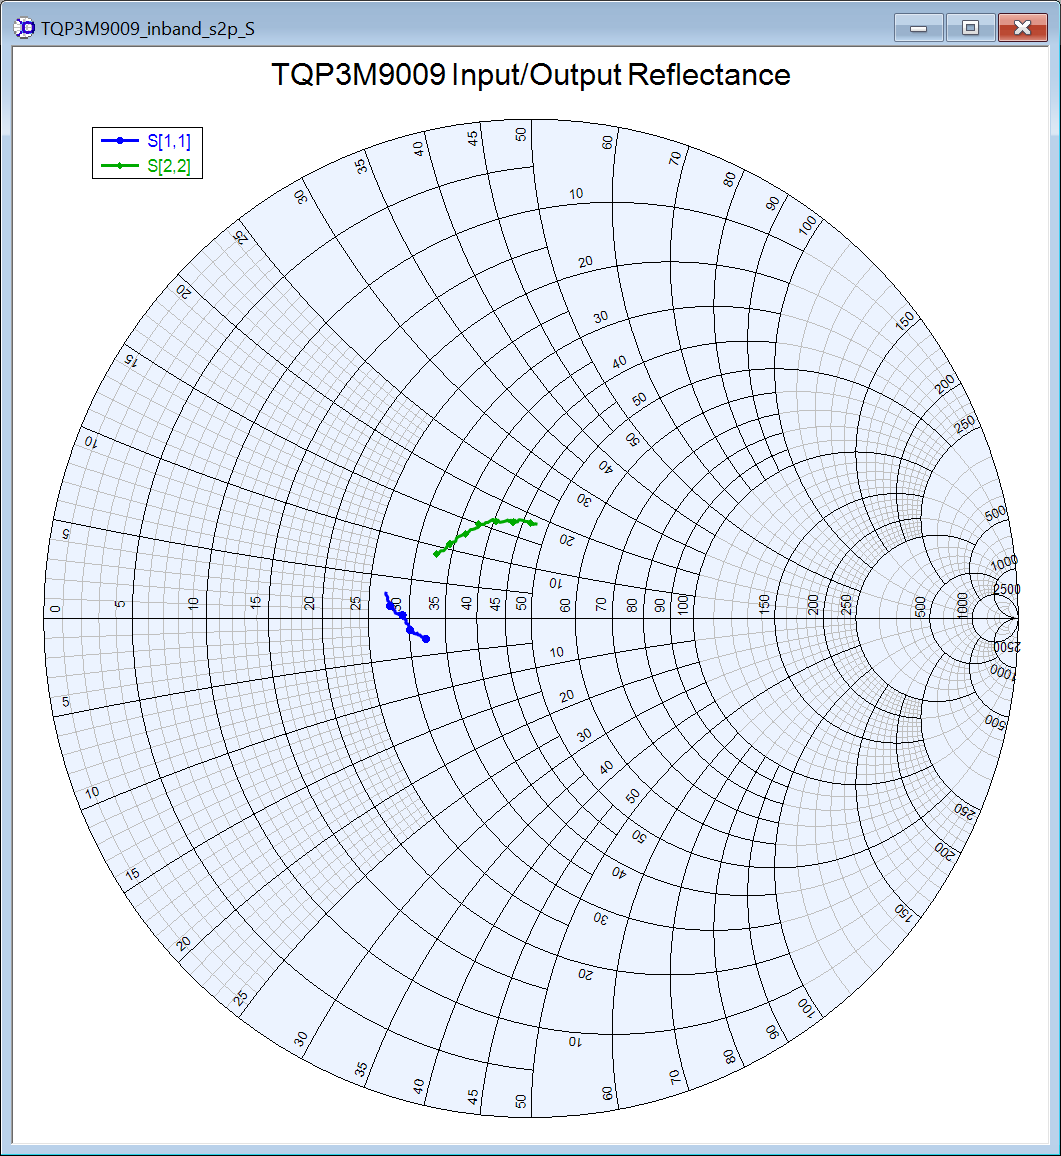
\includegraphics[width=0.44\linewidth]{figs/matching/TQP3M9009_smith}   \label{fig_tqp_smith}
        	}
	\subfigure[RFPA3800 Reflection Coefficients.]{
		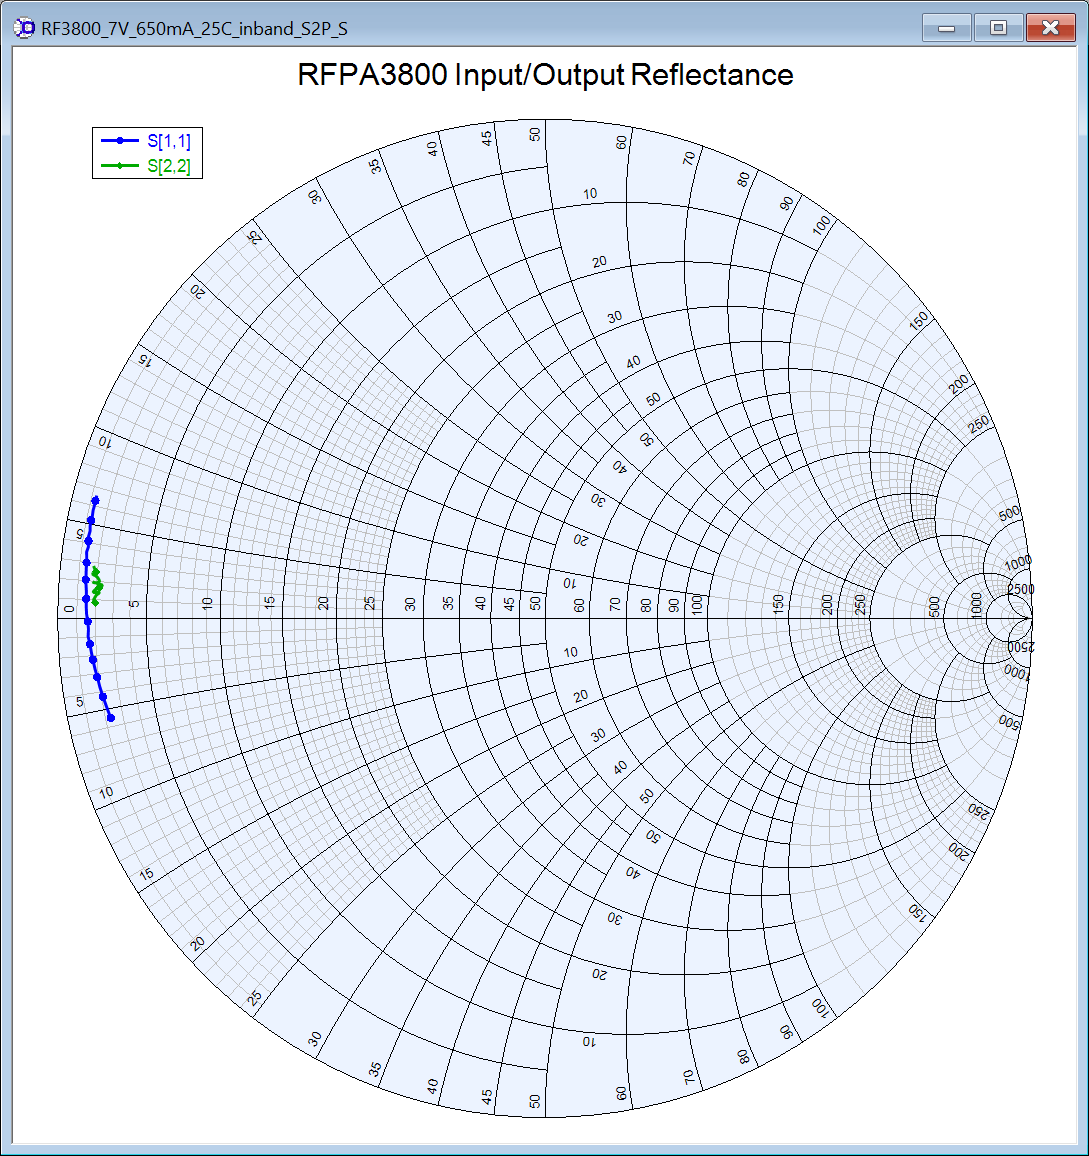
\includegraphics[width=0.45\linewidth]{figs/matching/RFPA3800_smith}   \label{fig_rfpa_smith}
        	}
\caption{Unmatched Smith Chart plots of PA components from 300 - 800 MHz.\label{fig_smith_charts}}
\end{figure*}
	
\subsubsection{Results for TQP3M9009}

	We display the results of the tuned optimization for the TQP3M9009 component in Figure~\ref{fig_srft_tqp}, with the \ac{MAG} (Equation~\ref{eq_mag}) displayed as an upper bound on the achievable matched gain for both the input and output matching circuits.
	In each case, we choose $T_{01} = T_{02} = 25$~dBm as the target flat gain value, represented as the flat dotted green line in Figure~\ref{fig_srft_tqp} (top left, top right).
	These values were chosen by trial and error as the maximum flat gain values that could be supported with this matching circuit.
		The number of matching elements is also chosen through trial and error in order to meet the optimization target with a minimal number of physical components.
		We can tell immediately from the relatively flat T1 and T2 \ac{MAG} that the TQP3M9009 is already well-matched and will require few components to produce a flat gain response.
		This is confirmed by viewing the Smith chart representation \cite{orfanidis2002electromagnetic} of the input and output reflection coefficients of the unmatched amplifier in Figure~\ref{fig_tqp_smith}, where we can see it is already well-matched in a 50~$\Omega$ system. 

	The resulting optimized TQP3M9009 gain with only input matching, $\text{T1}_{\text{dB}}$, and both input and output matching, $\text{T2}_{\text{dB}}$, is shown as solid blue lines.
	Compared to the \ac{MAG}, which represents the optimal gain in the case where each frequency point is optimized individually without regard for a broadband match, our optimized flat passband gain performs quite well.
	
	The physical ideal circuits that realize this optimized gain are also shown in Figure~\ref{fig_srft_tqp} (middle left, middle right).
	Numerical solutions to Equation~\ref{eq_stage_1} result in arbitrary circuit component values, but lumped elements are only available in discrete values.
	Therefore we perform a final processing step to round the solution lumped element component values to their nearest commercially available common values.
	The raw solution and the processed solution based on common component values is given as the second and third rows in Figure~\ref{fig_srft_tqp}.


%\pagebreak


\begin{figure}[p]
\centering
  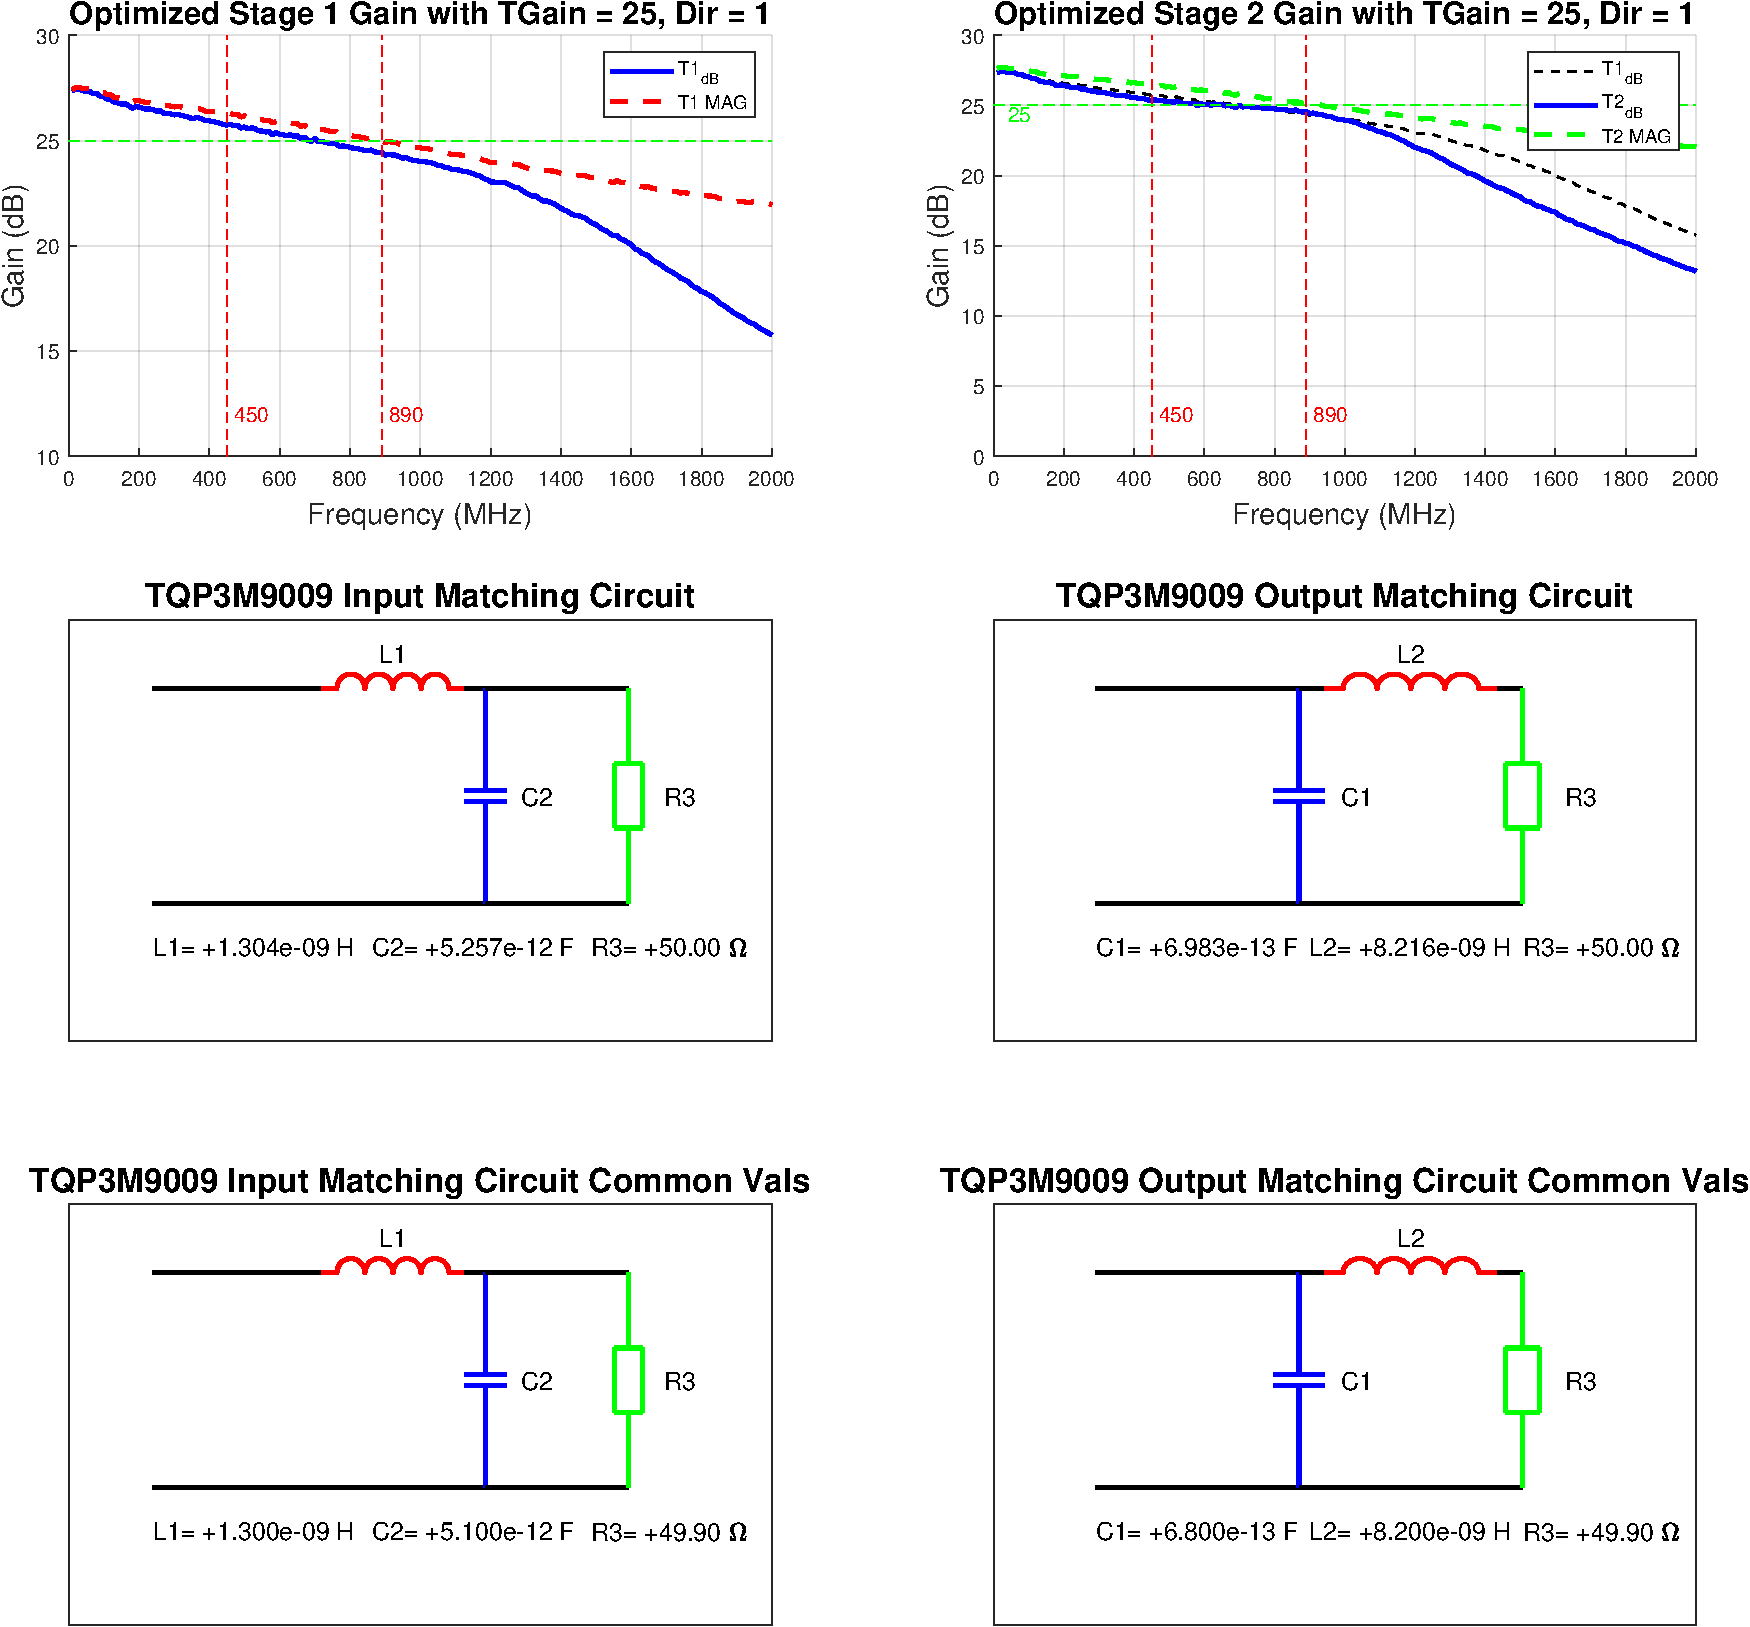
\includegraphics[width=1\linewidth]{figs/matching/14-Oct-2018_TQP3M9009_srft_results_sequential}   
    \caption{50-$\Omega$ input and output broadband match and synthesized circuit for 1st stage TQP3M9009 amplifier.}
\label{fig_srft_tqp}
\end{figure}


\pagebreak


%
%
%\begin{equation}
	%\argmax_{\textbf{[E]}}{T(\omega)} = |G_{21}|^2\frac{|E_{21}|^2}{|1-E_{11}G_{22}|^2|1-\hat{E}_{22}L_{11}|^2}|L_{21}|^2
%\end{equation}

\subsubsection{Results for RFPA3800}

	We display the results of the same tuned optimization for the RFPA3800 component in Figure~\ref{fig_srft_rfpa}, with the \ac{MAG} (Equation~\ref{eq_mag}) displayed as an upper bound on the achievable matched gain for both the input and output matching circuits.
	
	In this case, we empirically choose $T_{03} = 7.8$ and $T_{04} = 15.3$~dBm as the target flat gain value, represented as the flat dotted green line in Figure~\ref{fig_srft_rfpa} (top left, top right).
		
	The RFPA3800 presents a more difficult circuit to match; from its unmatched Smith Chart representation in Figure~\ref{fig_rfpa_smith} it is not internally matched to a 50~$\Omega$ system.
	This is a common occurrence with most high-power amplifiers or transistors, which leaves flexibility to the microwave designer, but also means we will need to apply more effort to get the part matched to 50~$\Omega$.

	This means that there is a larger different between the RFPA3800 T3 and T4 \ac{MAG} and its optimized flat gain, as shown in Figure~\ref{fig_srft_rfpa} (top left, top right).
	For the same reason, a larger number of matching components are required to achieve a reasonable flat frequency response across the band from 470 - 700~MHz and a few dB of gain compared to the upper bound \ac{MAG} are sacrificed in order to achieve this relatively flat gain target.
	
	We extended the upper frequency range in our final optimization of this broadband matching circuit to 800~MHz based on our experience implementing the circuit and finding that high-band performance above 650~MHz suffered from parasitics.
	This extra effort extends the lowpass roll off of the power transfer circuit topology higher to ensure that performance below 700~MHz remains nominal once implemented as a physical circuit.

\begin{figure}[p]
\centering
  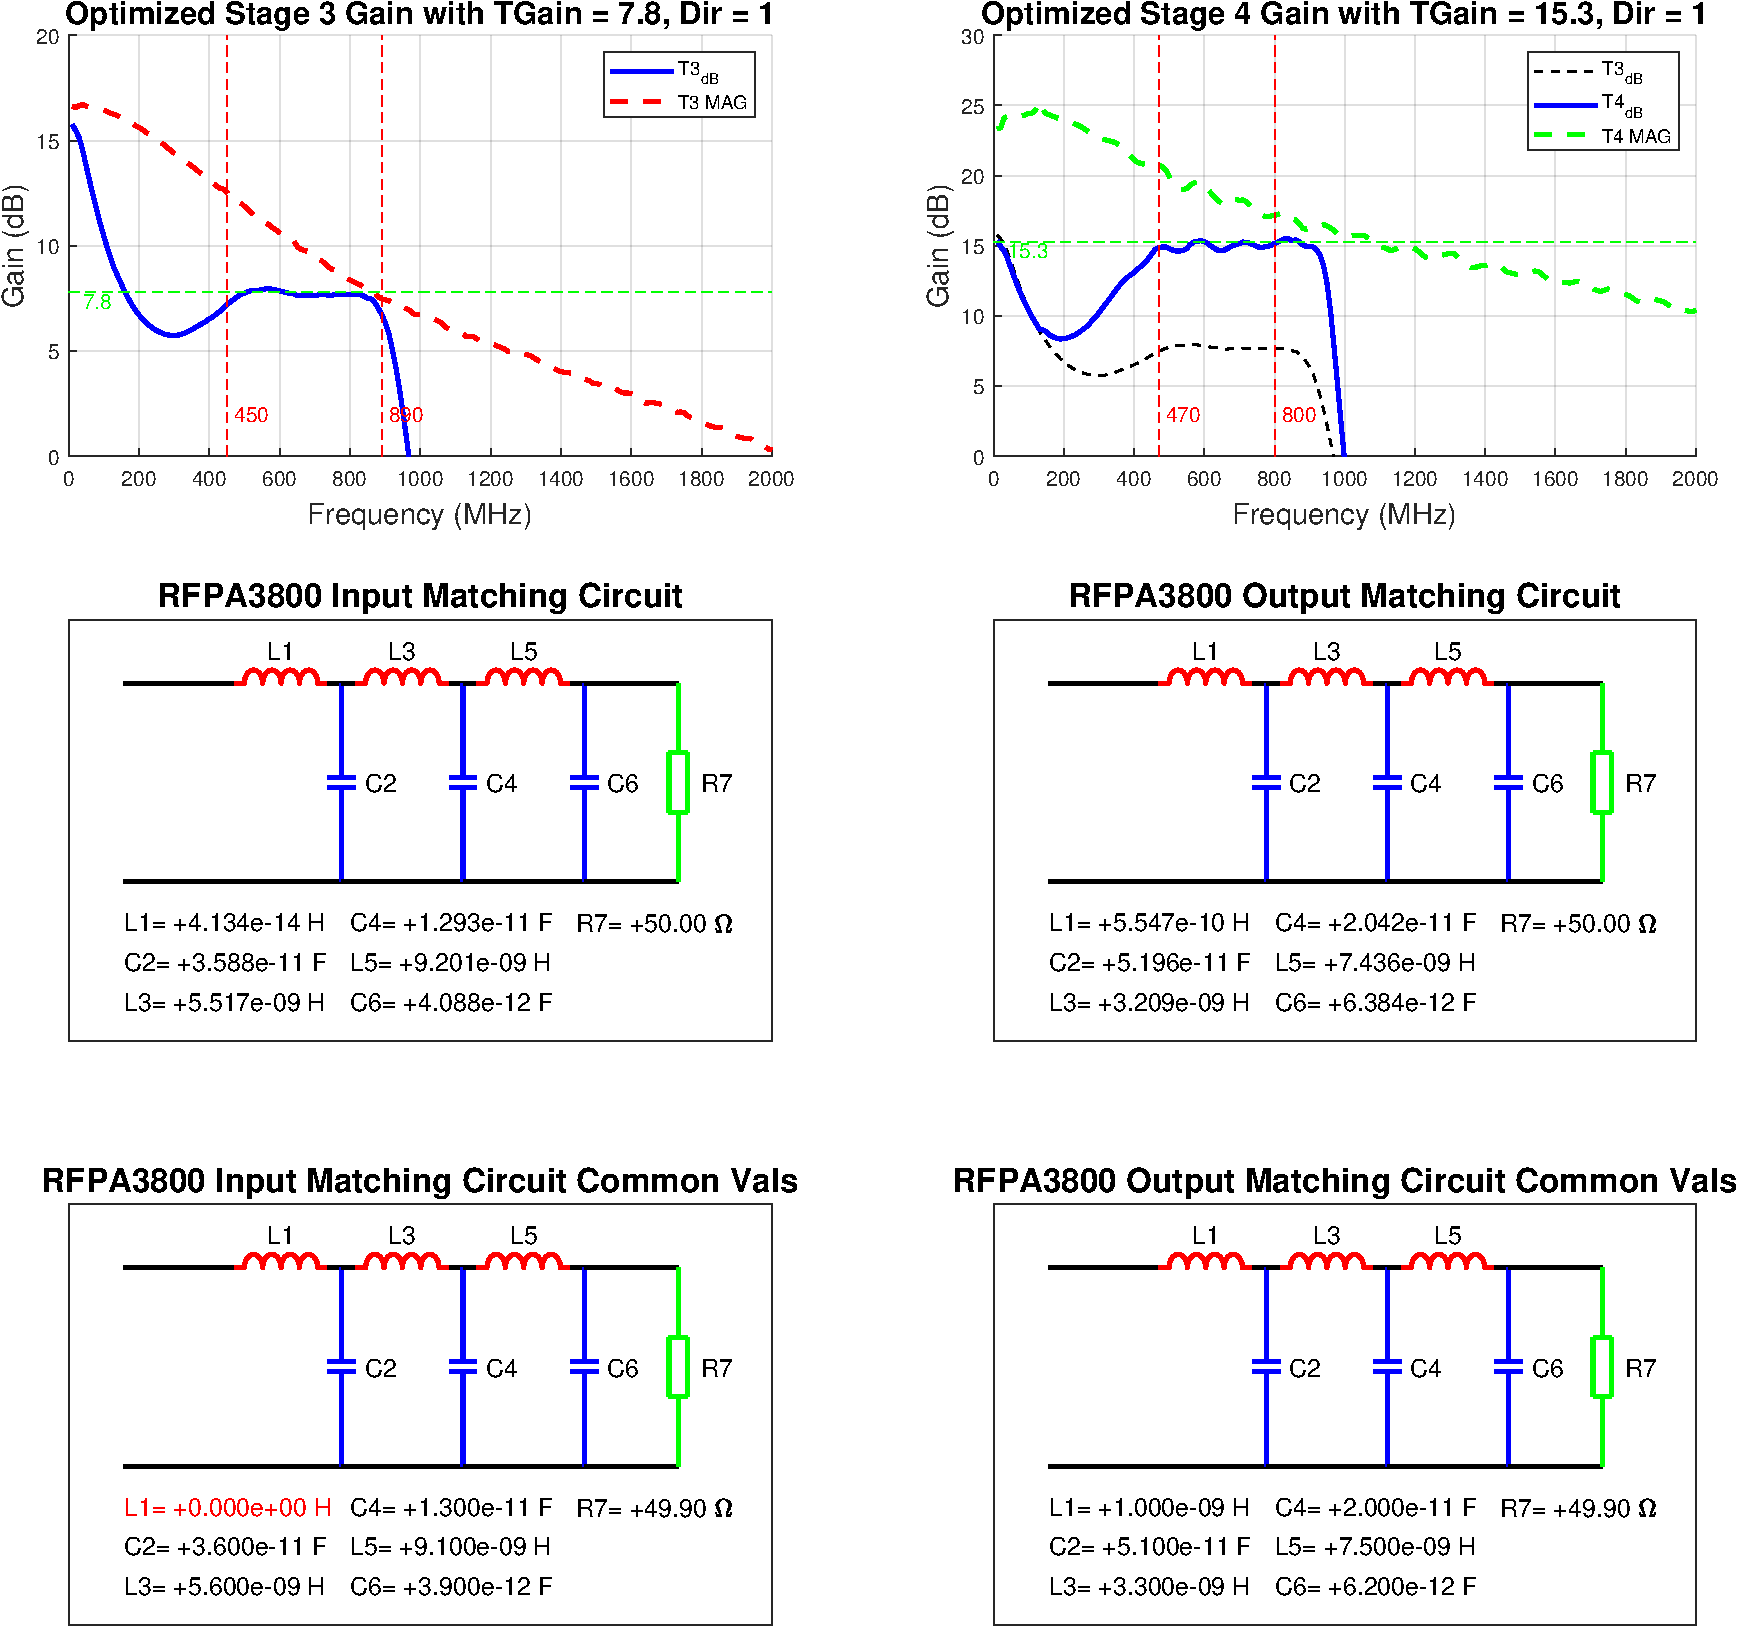
\includegraphics[width=1\linewidth]{figs/matching/14-Oct-2018_RFPA3800_srft_results_sequential}   
    \caption{50-$\Omega$ input and output broadband match and synthesized circuit for 2nd stage RFPA3800 amplifier.}
\label{fig_srft_rfpa}
\end{figure}


\pagebreak


%\begin{figure}[h]
%\centering
  %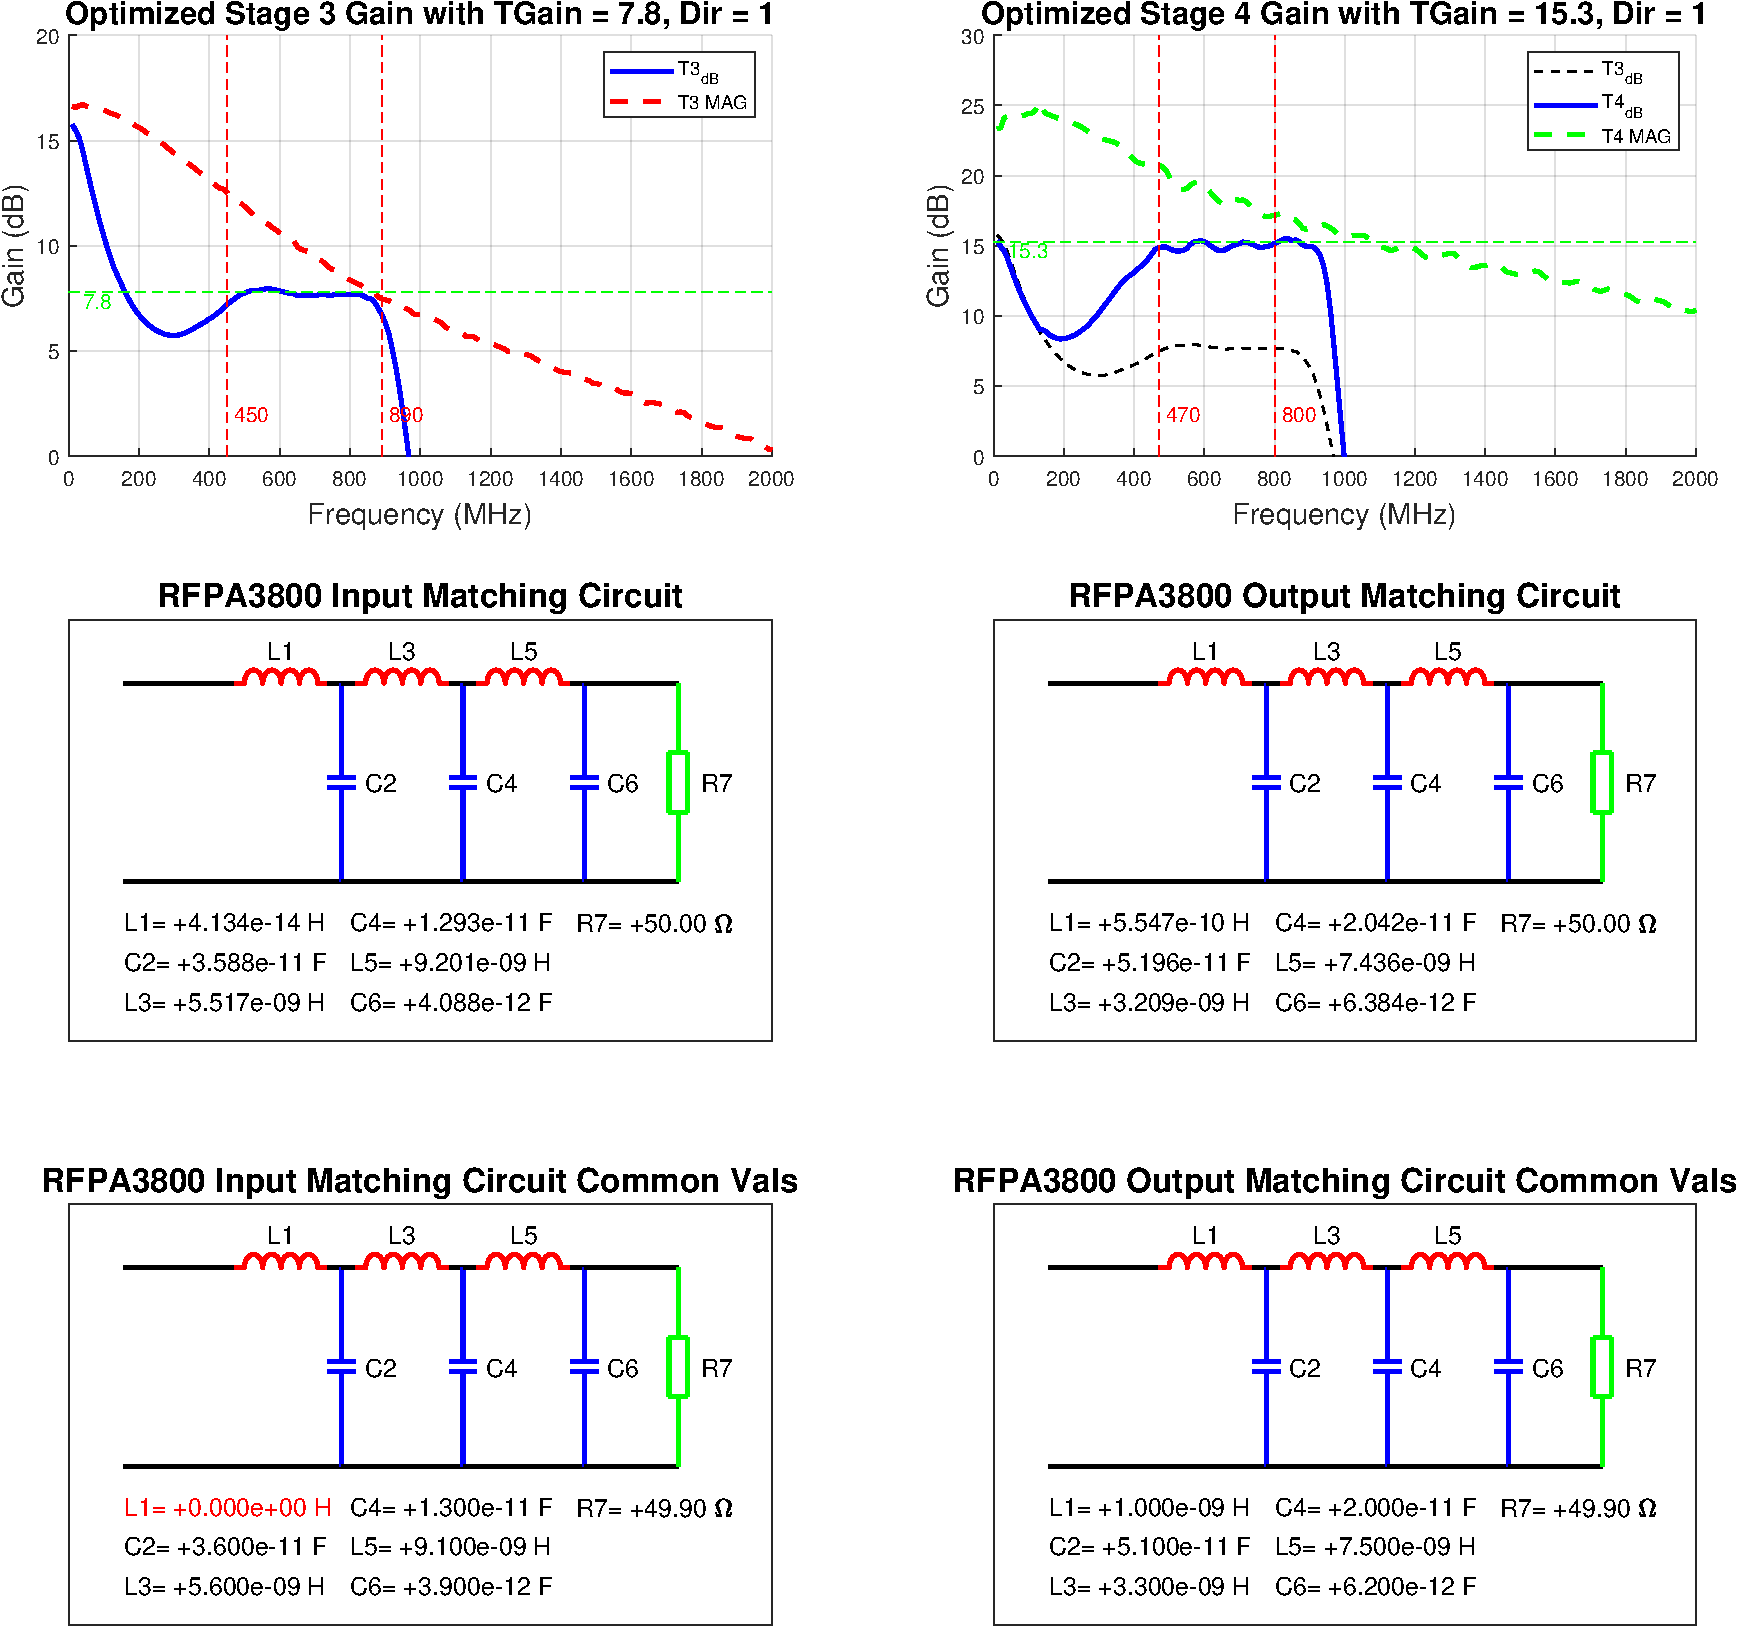
\includegraphics[width=0.9\linewidth]{figs/matching/14-Oct-2018_RFPA3800_srft_results_sequential} 
    %\caption{50-$\Omega$ input and output broadband match and synthesized circuit for RFPA3800 amplifier.}
%\label{fig_srft_rfpa}
%\end{figure}


%##################################################
\subsection{Simulation of Broadband Matching Networks}
\label{sec_broadband_ideal}
% XSPICE simulation circuit and results

%\begin{figure}[h]
%\centering
  %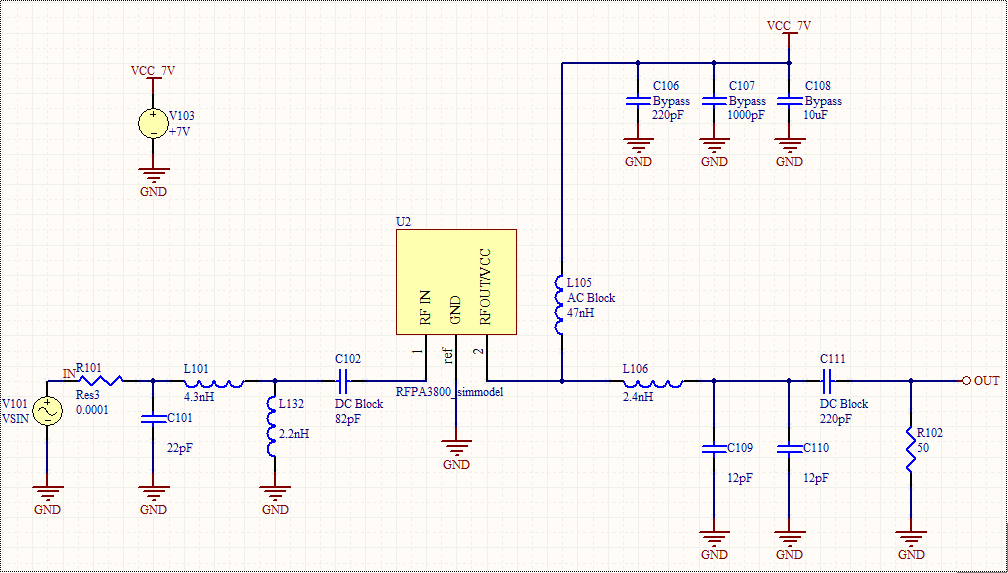
\includegraphics[width=4in]{figs/matching/RFPA3800_circuit}   
    %\caption{SPICE simulation circuit for ideal broadband power transfer network}
%\label{fig:tx_power_plot}
%\end{figure}

	In this section, we present an early prototype of the \ac{WURC} broadband power transfer network that utilized the same real frequency numerical optimization design technique as discussed in Section~\ref{sec_srft_stage_1} and \ref{sec_srft_stage_2}, but rather than matching each amplifier to a 50~$\Omega$ input and output impedance, the multiple stages were cascaded into each other following the general procedure outlined in Yarman 1982 \cite{yarman1982simplified}.
	The intent of these simulations were to confirm the validity of the designed broadband matching circuit before producing physical prototypes; however we found that both our design technique as well as our modeling approach was insufficient to fully represent the physical realization of the broadband matching circuit.
	In this section we will discuss in detail why this occurred and the additional steps needed to implement the ideal broadband power transfer network developed in Section~\ref{sec_dual_match}.

	The initial prototype circuit design is shown in Figure~\ref{fig_spice_circuit}, where XSPICE models for the amplifier elements were extracted from the empirical S-parameter files using EMtoSPICE \cite{mandrutareduced}, a commercial tool for extracting stable time-domain simulation models from frequency-domain S-parameter data.
	We used the built-in XSPICE simulator in \ac{CAD} tool Altium Designer 13 to simulate the steady-state frequency response of the broadband amplifier chain.
	In Figure~\ref{fig_spice_results}, we show the broadband matching gain as a function of the center frequency.
	Both a match to a 65~$\Omega$ (blue) and 50~$\Omega$ (red) differential source impedance were simulated, as we had not yet decided how to compensate for the LMS6002D's 65~$\Omega$ source impedance.
	
	With a minimum simulated 39.2~dBm in-band gain matched against a 50~$\Omega$ source, this was sufficiently close to the designed frequency response that a prototype \ac{PCB} was fabricated to implement the circuit for testing and fine-tuning.
	
% SPICE Model Circuit
\begin{figure}[p]
\centering
  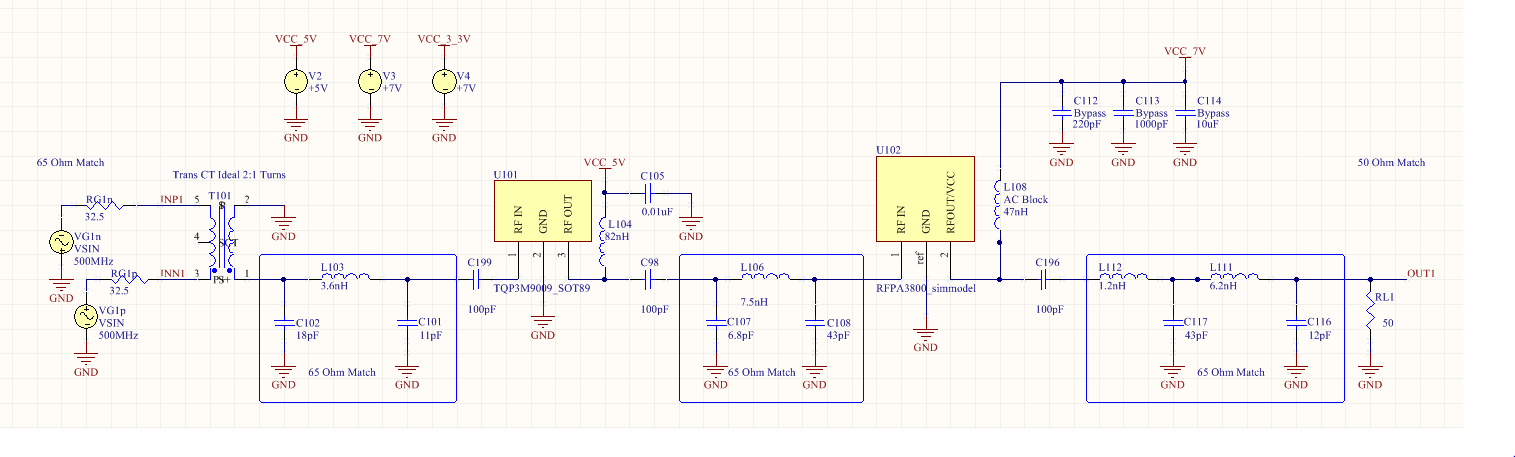
\includegraphics[width=1\linewidth]{figs/matching/tqp_rfpa_circuit_50_65_load}   
    \caption{XSPICE simulation circuit for ideal broadband power transfer network.}
\label{fig_spice_circuit}
\end{figure}

% SPICE Simulation Results
\begin{figure}[p]
\centering
  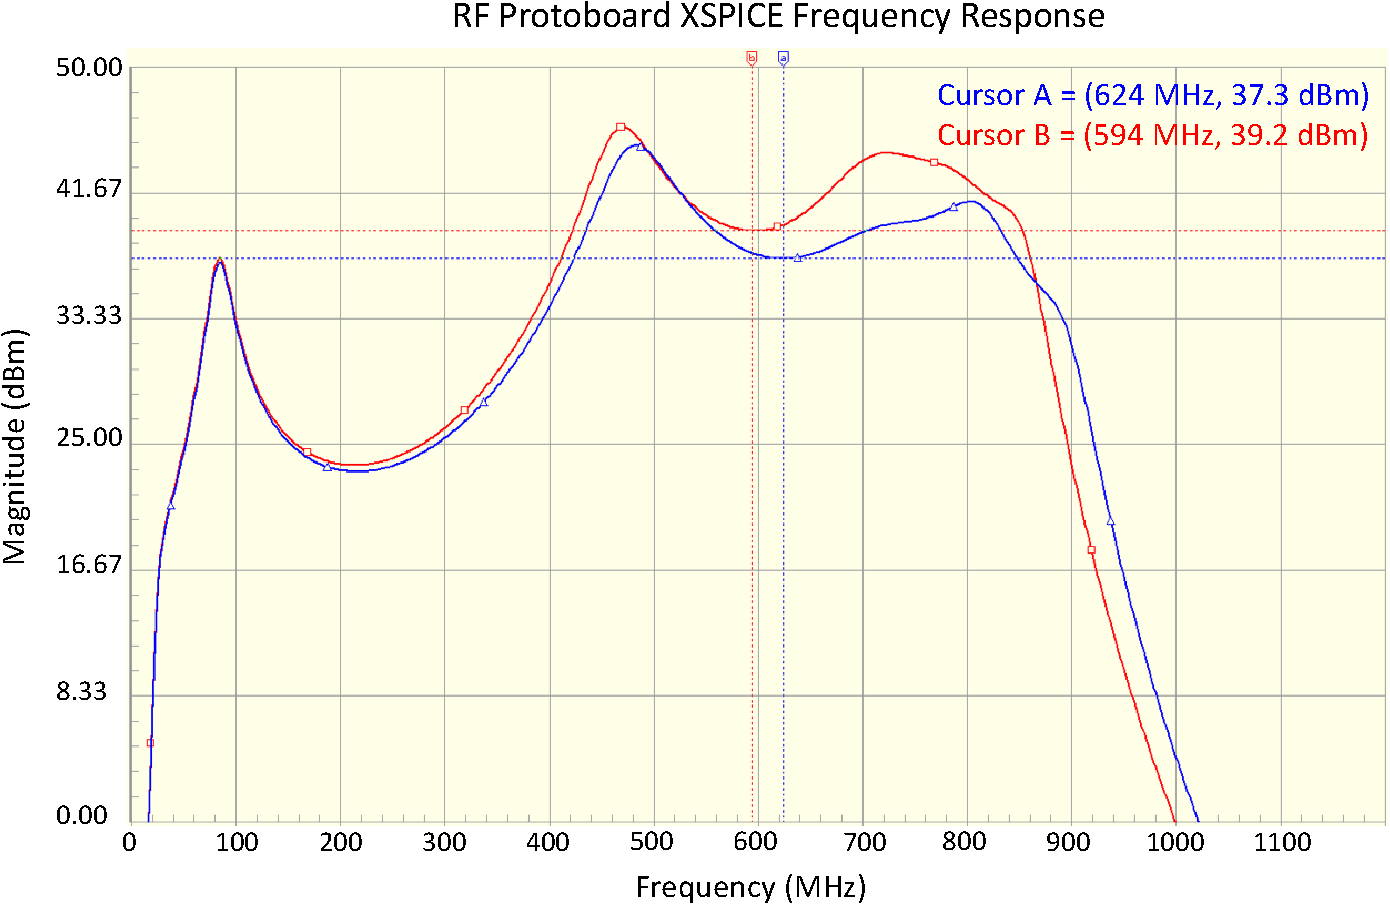
\includegraphics[width=0.9\linewidth]{figs/matching/RF_Protoboard_XSPICE}   
    \caption{XSPICE simulation results of ideal broadband power transfer network.}
\label{fig_spice_results}
\end{figure} 
	
% #########
\subsubsection{Evaluation of Broadband Matching Networks}
\label{sec_rf_protoboard}
% RF Protoboard and results
	
	We designed and manufactured a controlled impedance 2-layer PCB to implement the circuit presented in Figure~\ref{fig_spice_circuit} \ref{sec_broadband_ideal}.
	With 50~$\Omega$ input and output, the circuit was designed to provide space for any additional matching components and RF probes.
	%An additional pass-through 50~$\Omega$ microstrip trace was provided to de-embed the PCB or individual components, should that become necessary.
	The assembled PCB is shown in Figure~\ref{fig_match_proto_pcb}.
	The extra grounding copper foil shown in the picture was added after initial characterization and can be ignored.
	
	The prototype amplification PCB was measured with a calibrated vector network analyzer and it became clear that the physical device performance was not matching simulated results.
	We show the actual $|S_{21}|$, or forward gain, of the cascaded designed gain stages in Figure~\ref{fig_match_proto_gain}, where we can immediately see that gain unexpectedly drops off to zero drastically after approximately 500~MHz whereas the designed circuit maintained a flat gain out beyond 800~MHz in simulation.

% RF Prototype Board for UHF RF PAs
\begin{figure}[p]
\centering
  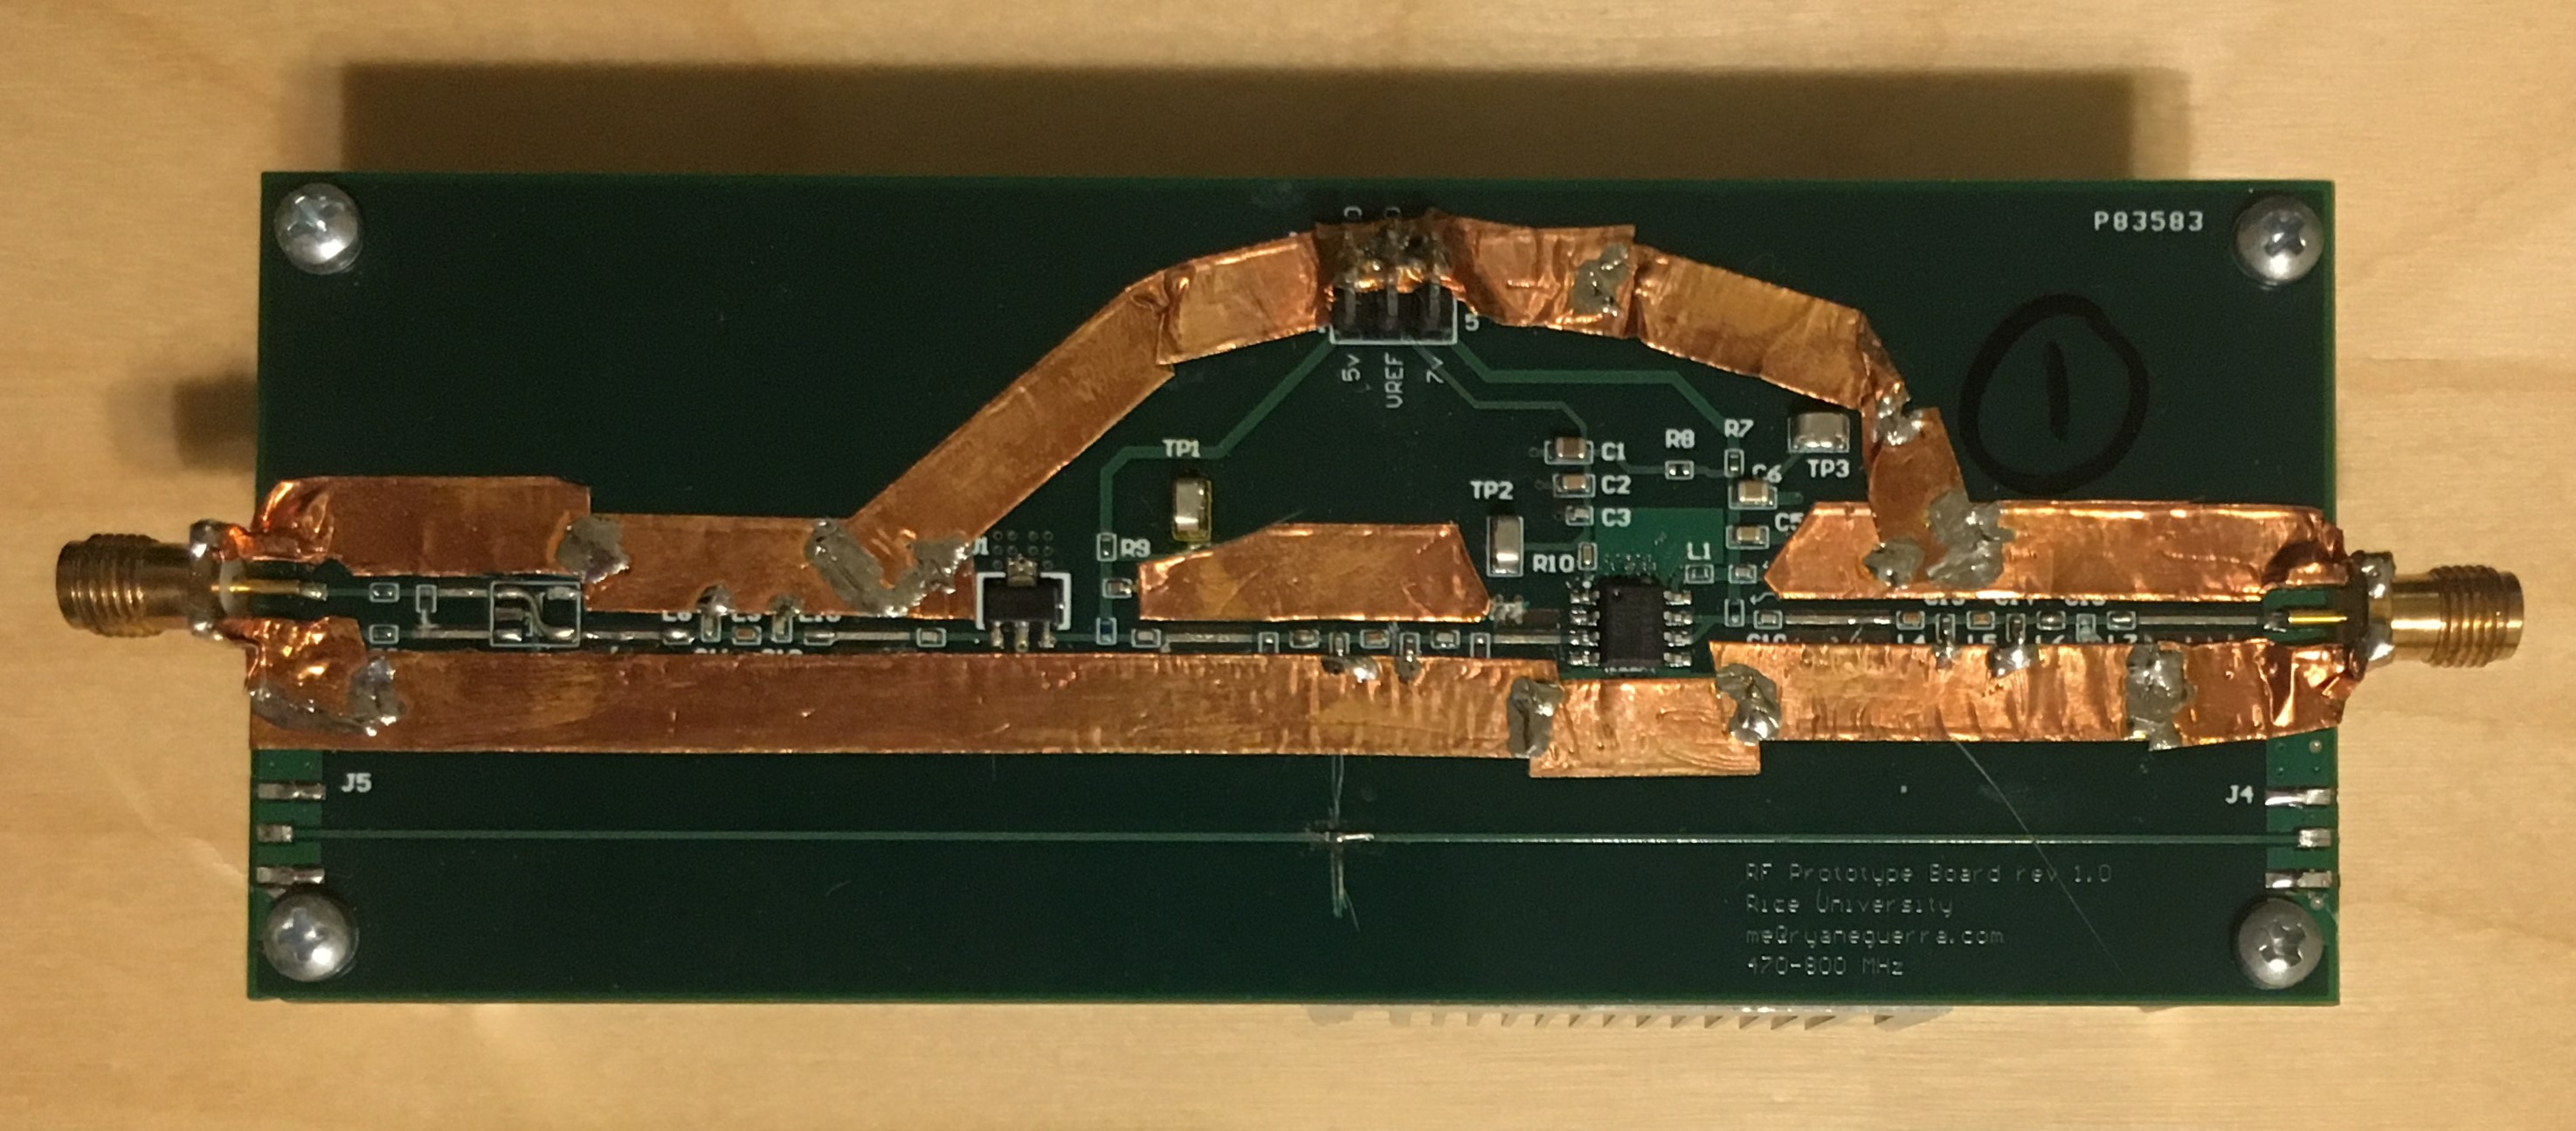
\includegraphics[width=1\linewidth]{figs/matching/rf_protoboard}   
    \caption{Prototype PCB of WURC broadband power transfer circuit.}
\label{fig_match_proto_pcb}
\end{figure}

% Gain Plot for RF Prototype Board
\begin{figure}[p]
\centering
  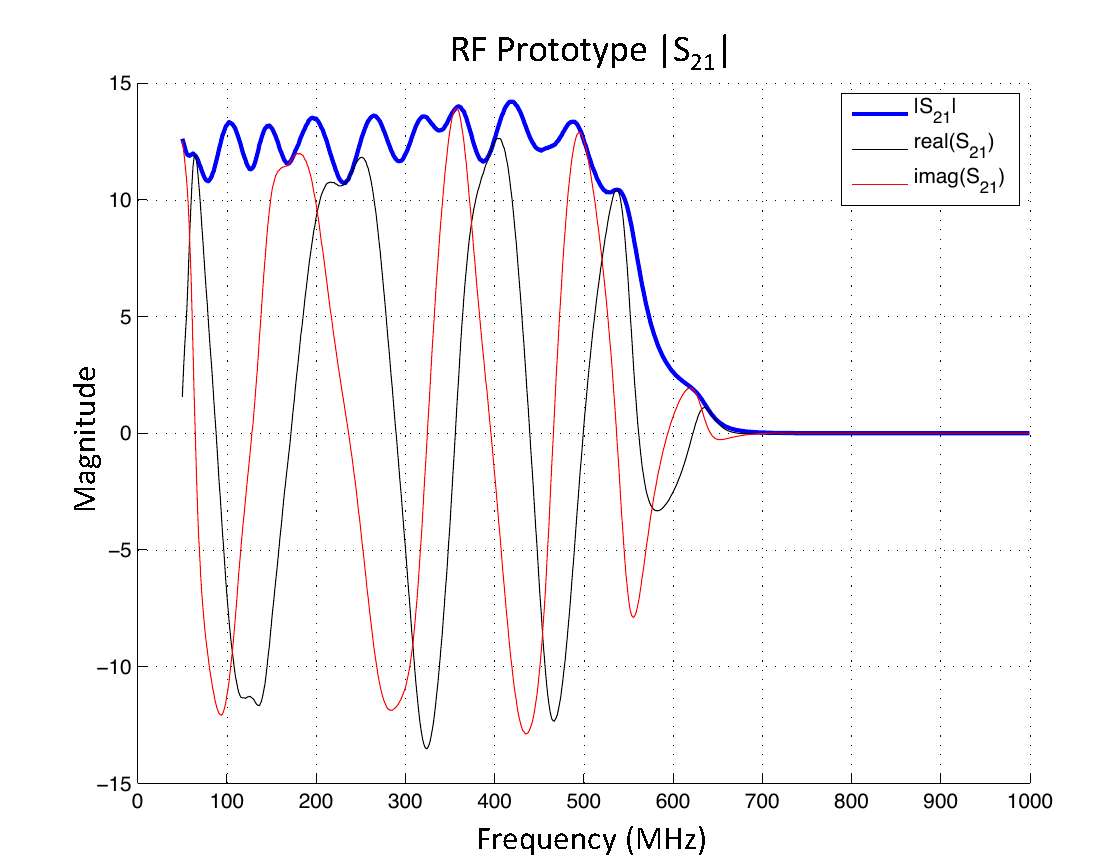
\includegraphics[width=0.8\linewidth]{figs/matching/RF_Protoboard_S21_measured}   
    \caption{Measured gain of prototype WURC broadband power transfer circuit.}
\label{fig_match_proto_gain}
\end{figure}


	The root cause of this unintended result is the inability of the real-frequency matching technique to directly consider parasitic circuit elements in its formulation.
	It is a well-characterized fact that physical circuit elements are non-ideal: coupling between physical elements and construction from non-ideal materials yields parasitic resistance, capacitance, and inductance in each lumped-element component.
	A chip capacitor in particular has a \ac{SRF}, $\omega_0 = \frac{1}{\sqrt{L_p\cdot C}}$, when the desired series capacitance resonates with the parasitic series inductance of the part \cite{murata2010srf}.
	Below the resonant frequency, the capacitance term dominates; above the resonant frequency, the parasitic inductive term dominates and the physical capacitor no longer behaves like an ideal capacitor.
	
	\pagebreak
	
	For example, we present the empirical impedance functions provided by the component manufacturer of three chip capacitors considered in our matching circuit design in Figure~\ref{fig_cap_comparison}: a 16~pF 0201 (GRM0335C1H160 blue), a 5~pF 0402 (GJM1555C1H5R0 green), and a 47~pF 0402 (GJM1555C1H470 red).
	These capacitors were considered to implement the circuit in Figure~\ref{fig_spice_results}, specifically component C117 in that diagram.
	
	The 47~pF 0402 component has a self-resonant frequency of approximately 1600~MHz, represented by the trough in the red curve in Figure~\ref{fig_cap_comparison}.
	As a rule of thumb, the \ac{SRF} of a component should be selected to be approximately 3-times larger than the maximum operating frequency of the circuit for filters and matching application in order to ensure that its behavior approaches its expected ideal behavior.
	We confirmed that this particular capacitor was behaving in a non-ideal manner due to its low \ac{SRF} that effectively destroyed the designed conjugate match above 500~MHz in the implemented circuit.
	
	In general, larger value capacitances and larger physical packages result in lower \ac{SRF}, so we focused on reducing both parameters.
	
% Self-resonant frequencies for capacitors in WURC
\begin{figure}[hb]
\centering
  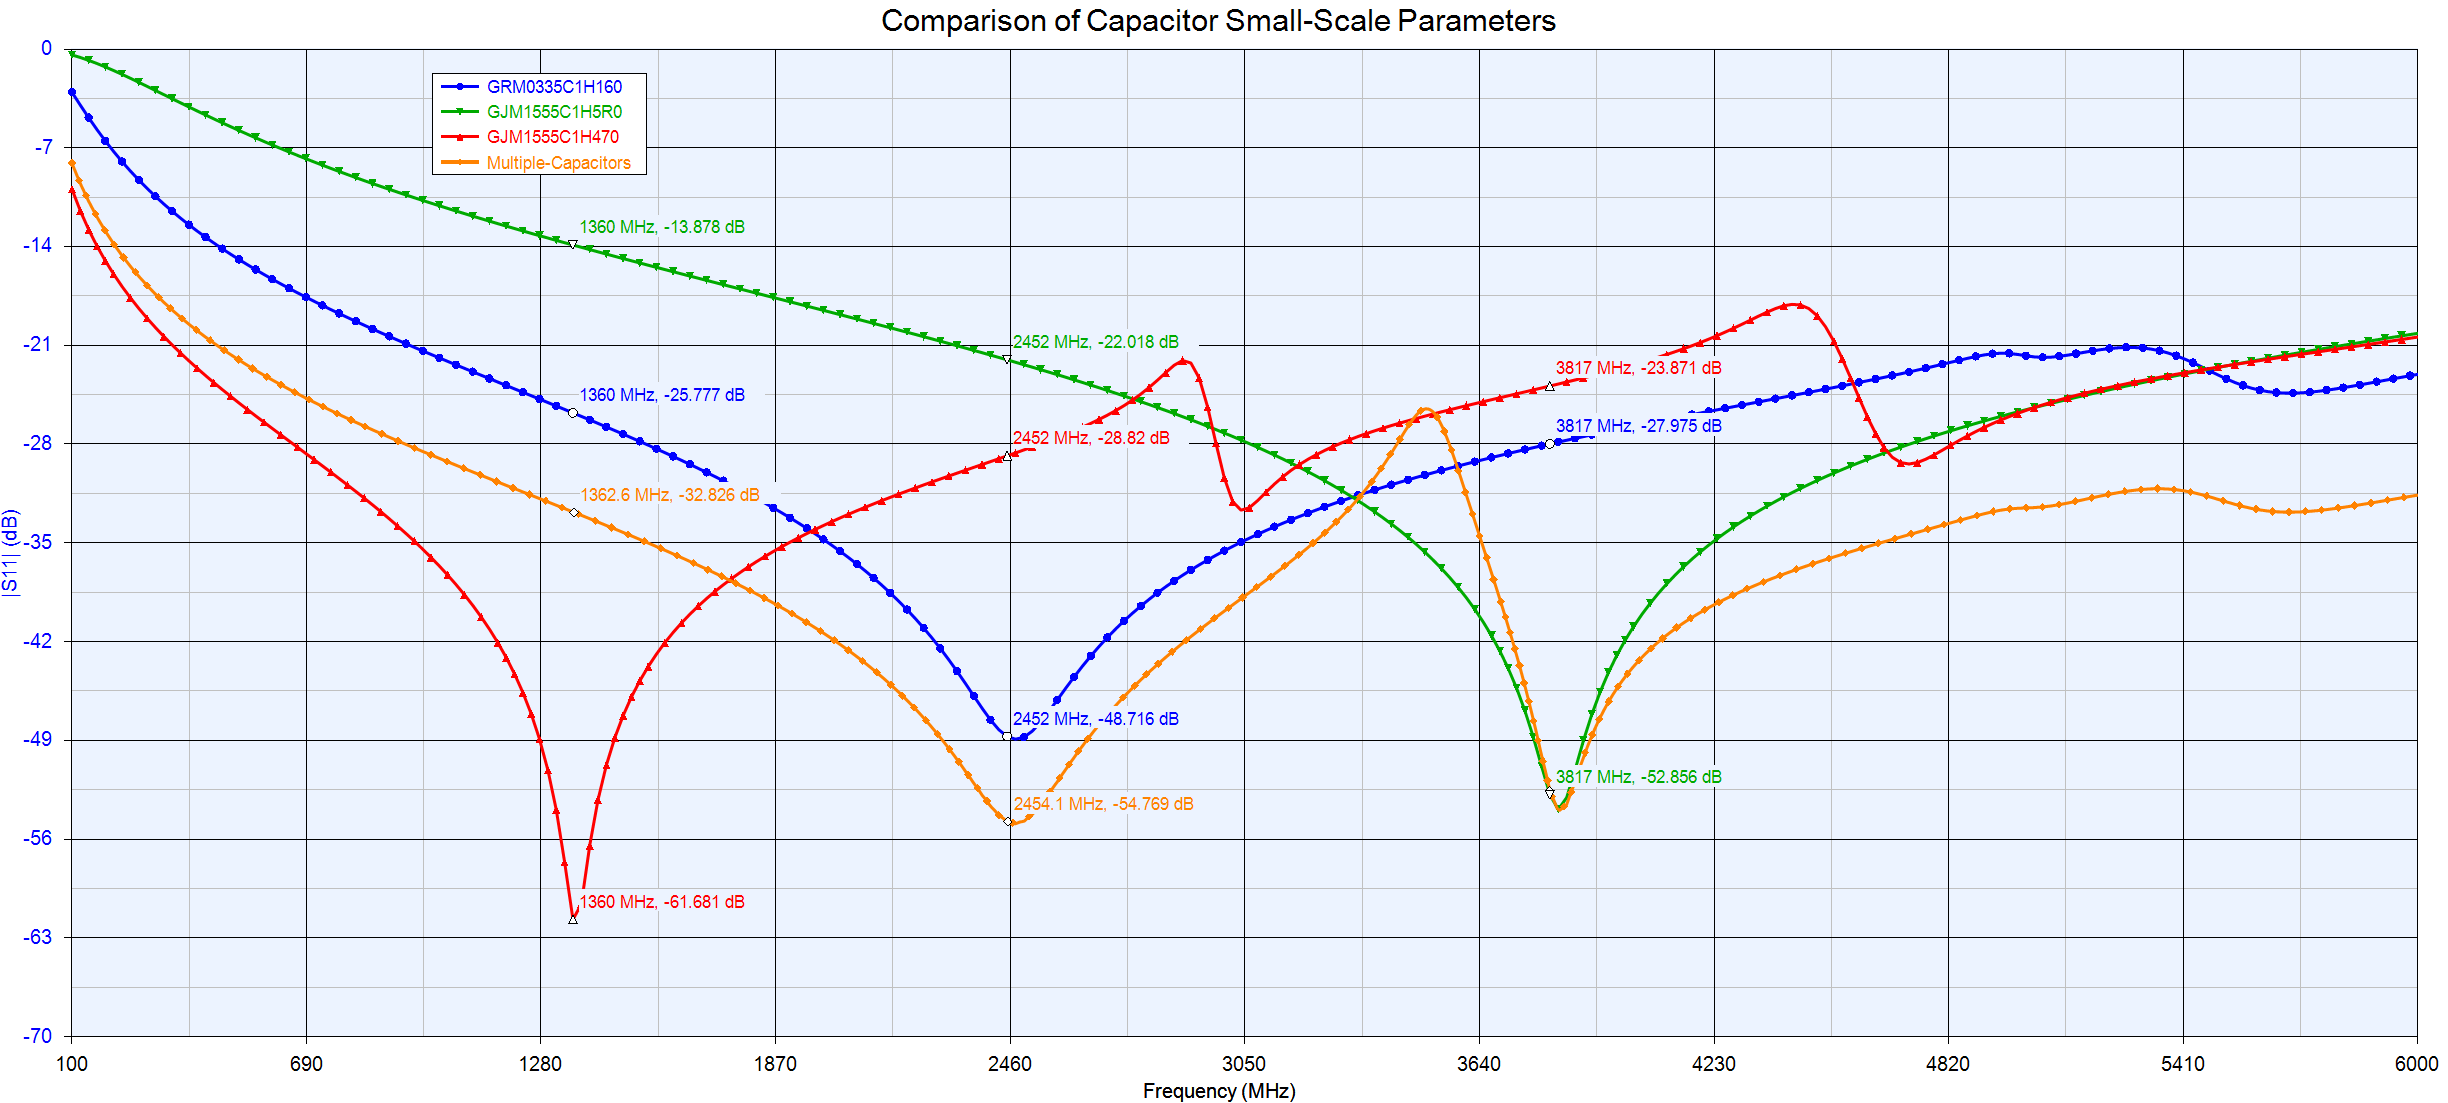
\includegraphics[width=1\linewidth]{figs/matching/capacitor_comparison}   
    \caption{S-parameters for various MLCC capacitor configurations.}
\label{fig_cap_comparison}
\end{figure}
	
	After much iteration with small-scale simulation techniques that could accurately model the parasitics, we decided to replace the 47~pF 0402 with three different capacitors in parallel: two 16~pF 0201 and one 5~pF 0402 capacitor.
	The \ac{SRF} for these two parts was respectively 2450~MHz and 3820~MHz, well above the maximum 800~MHz operating range of the amplifiers; the combined frequency response of this parallel circuit is shown in Figure~\ref{fig_cap_comparison} as the orange plotline.
		

%##################################################
\subsection{Simulation of Broadband Matching Networks with Parasitics}
\label{sec_wurc_parasitics}

	While this design was confirmed at the early design stage with XSPICE simulation models, evaluation of the prototypes presented earlier demonstrated that package parasitics in the lumped-element broadband power transfer chain were missing from the XSPICE simulator models.
	These parasitics severely impaired the implemented high-frequency gain response above 500~MHz and required a more advanced model and simulation technique to correctly predict their effect.
	Re-modeling the RF chain in the Cadence Virtuoso SpectreRF circuit simulator utilizing empirical S-parameter models resulted in a more accurate simulation, allowing package parasitics to be compensated for in the lumped-element design.

	We considered the entire physical layout in SpectreRF, including transformers, microstrip, switches and filters.
	For each discrete component, empirical S-parameter files were obtained from the equipment manufacturer or directly generated from development boards using a vector network analyzer.
	The resulting physical model considering parasitics and layout is shown in Figure~\ref{fig_spectre_uhf_circuit} for the entire \ac{WURC} UHF transmit chain.
	
% PAGEBREAK  vvvvvvvvvvvvvv
% SpectreRF full RF chain model
\begin{figure}[p]
\centering
  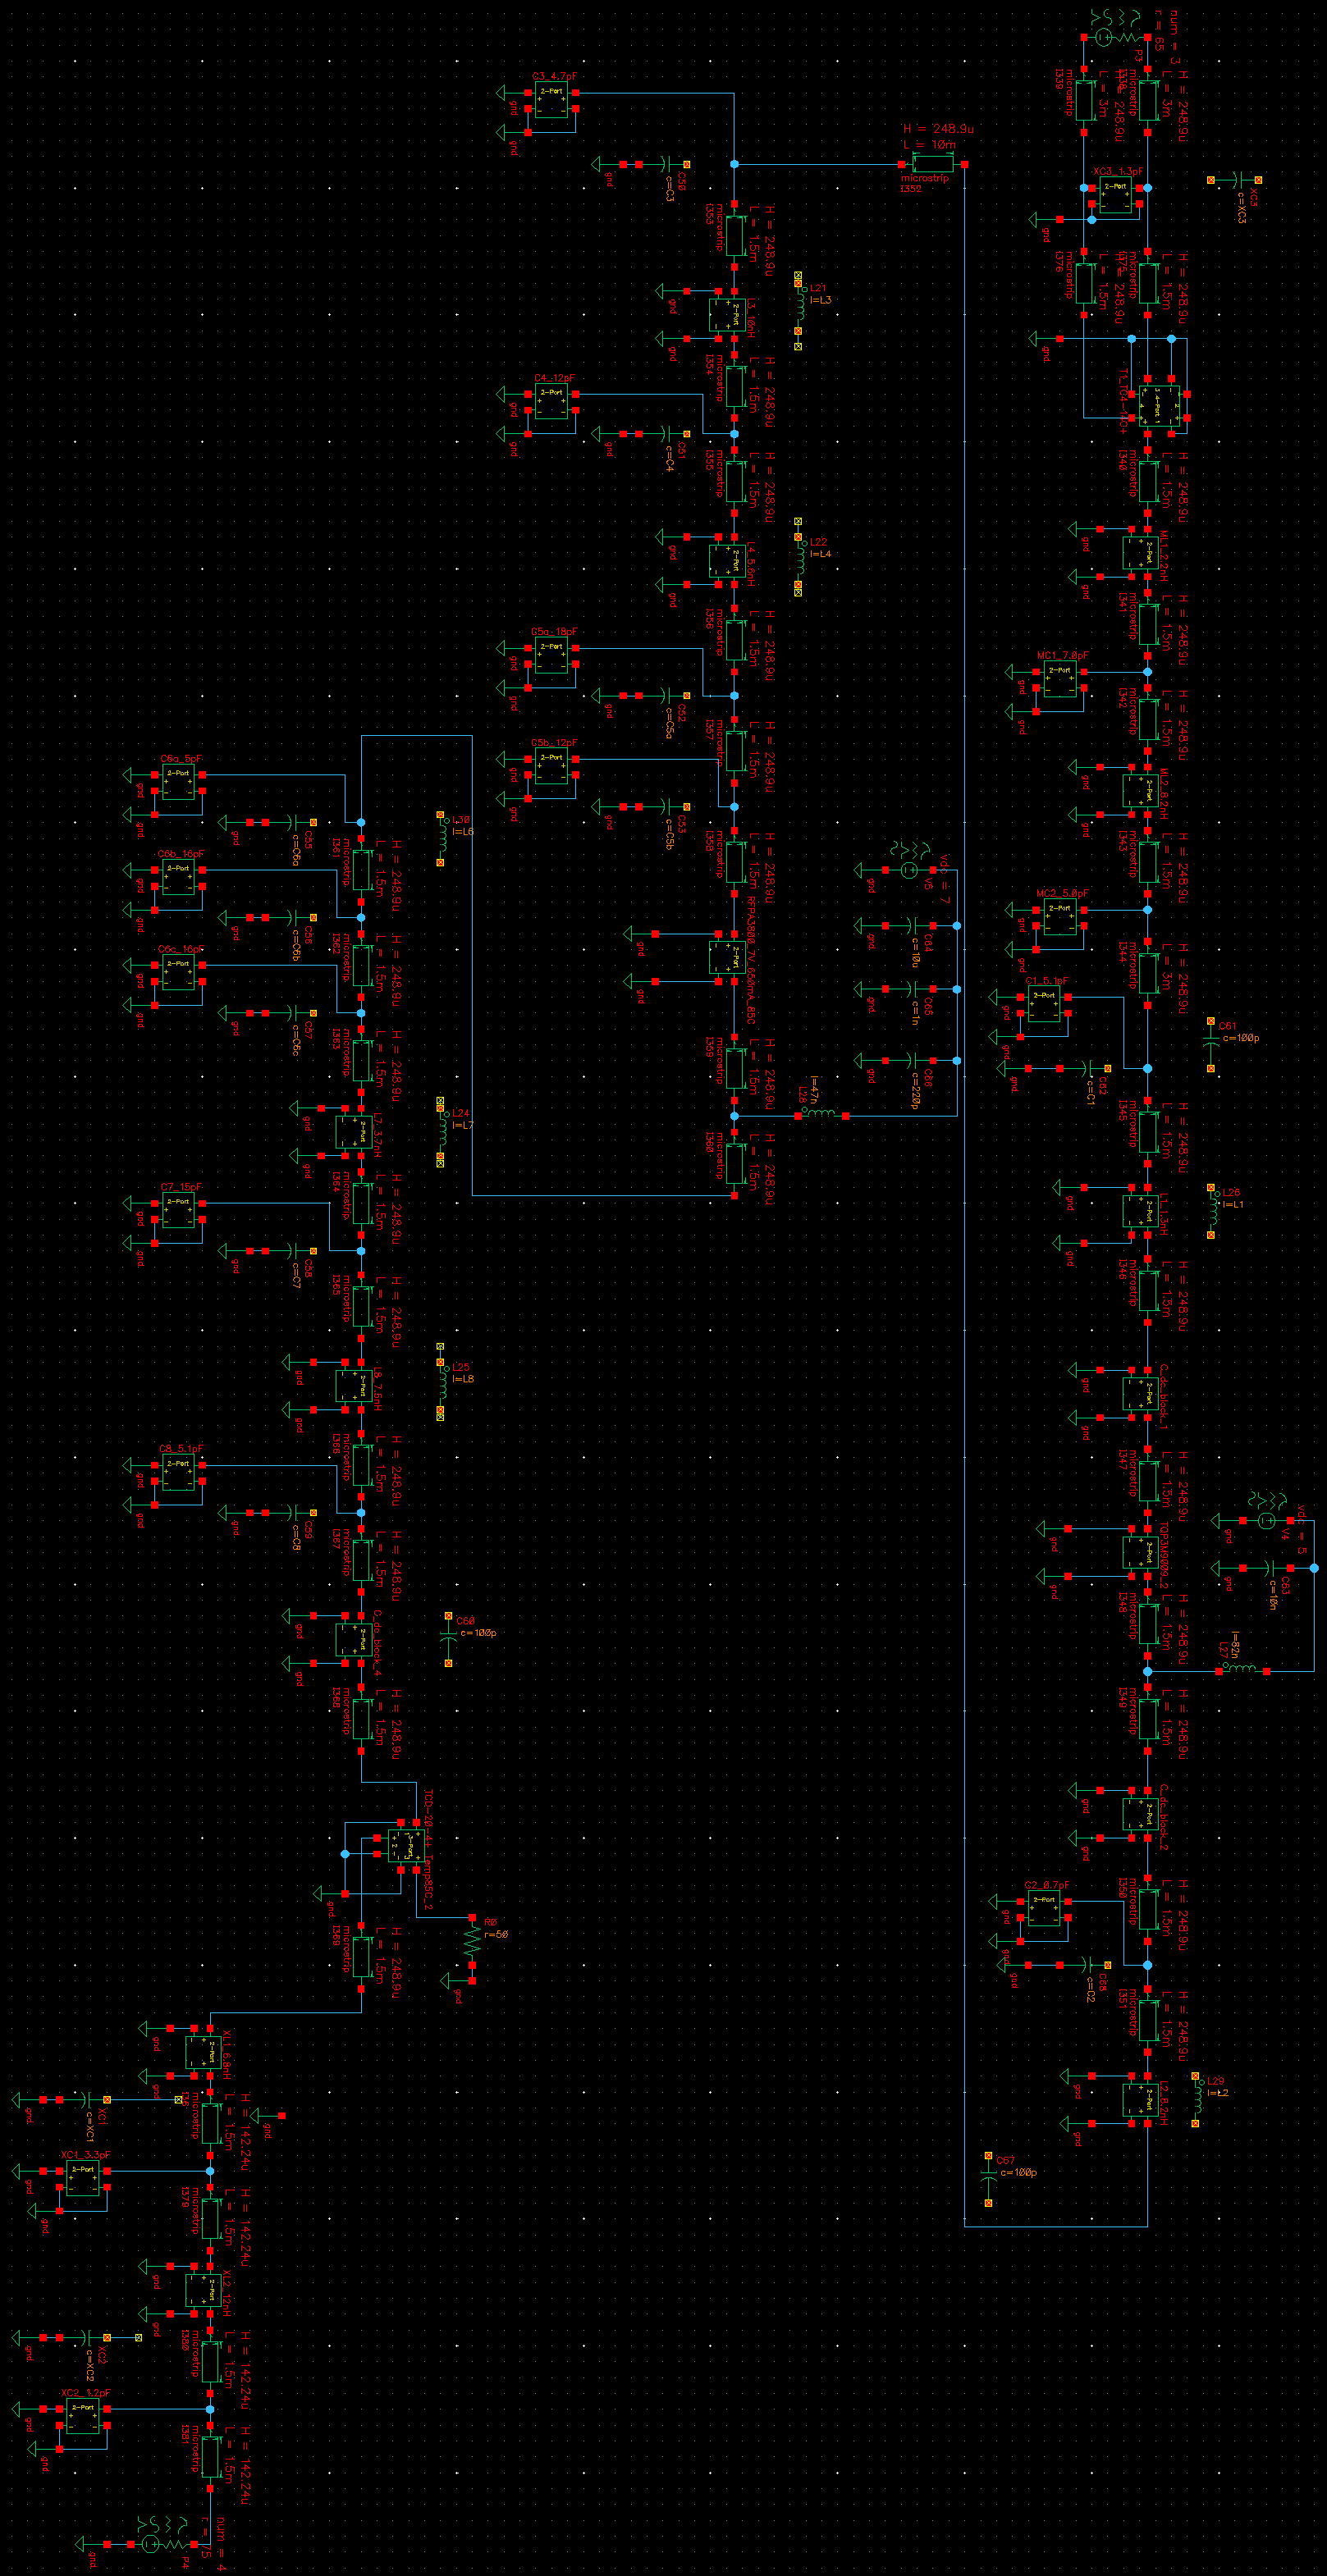
\includegraphics[width=0.75\linewidth]{figs/matching/spectre_uhf_tx_complete_chain}   
    \caption{Simulation model of full UHF transmit chain in Cadence Virtuoso SpectreRF.}
\label{fig_spectre_uhf_circuit}
\end{figure}
% PAGEBREAK  ^^^^^^^^^^^^^^

	The simulated results for the SpectreRF system in Figure~\ref{fig_spectre_uhf_circuit} are shown in Figure~\ref{fig_spectre_uhf_results}.
	Here, we present two results: 1) the gain performance of the system where each lumped element is replaced with an ideal capacitor or inductor while all other active components, switches, and traces are modeled by their empirical representations with parasitics (red); and 2) the gain performance when each ideal component has been replaced with an empirical S-parameter model and hand-tuned individually to bring performance as close to the ideal as possible (green).
	
	The hand-tuning procedure is inherently greedy but produces satisfactory results: 
	\begin{itemize}
		\item \textbf{Step 1}: select an arbitrary ideal component, replace the ideal component with its S-parameter small-signal model;
		\item \textbf{Step 2}: replace this component with the small-signal model for a component with a smaller or larger common value (\emph{e.g.} a 9~pF capacitor would be compared with a 10~pF and 8~pF component in this step);
		\item \textbf{Step 3}: select the component with system frequency response that is most like the ideal system frequency response, set this component selection;
		\item \textbf{Step 4}: repeat from Step 2 until no improvement in the system frequency response is gained;
		\item \textbf{Step 5}: repeat from Step 1 until all ideal components have been replaced with small-signal models.
	\end{itemize}
	
	Since there are generally fewer inductor step sizes in commonly-available \ac{SMT} components than capacitor step sizes, we perform the greedy tuning algorithm first on all of the inductors in a model and \emph{then} on the capacitors.
	
	We can see that the final circuit frequency response in Figure~\ref{fig_spectre_uhf_results} has good, flat performance with only 4~dB ripple from 470 - 750~MHz, and that the modeled gain diverges by 2-3~dB from ideal modeled performance primarily at the high frequencies above 550~MHz.
	The overall system gain in the SpectreRF simulation in Figure~\ref{fig_spectre_uhf_results} is smaller than that predicted by XSPICE in Figure~\ref{fig_spice_results}, but it also considers losses from component parasitic resistances, switch and filter insertion loss, and microstrip losses and is closer to that of the physical circuit realization.
	
%##################################################
\subsubsection{Evaluation of Broadband Matching Networks with Parasitics}
\label{sec_wurc_parasitic_eval}
	
	Finally, having considered all physical impairments in our simulation model and after hand-tuning the simulated design, we realized this new circuit design in the first \ac{WURC} prototype shown in Figure~\ref{fig_wurc_versions} as the green PCB.
	Additional simple resistive impedance matches were made from the source LMS6002D 65~$\Omega$ differential to the system 50~$\Omega$ single-ended and from the system 50~$\Omega$ to the 75~$\Omega$ output antenna ports, but these were not difficult and the process is omitted here.

% SpectreRF simulation results
\begin{figure}[ht]
\centering
  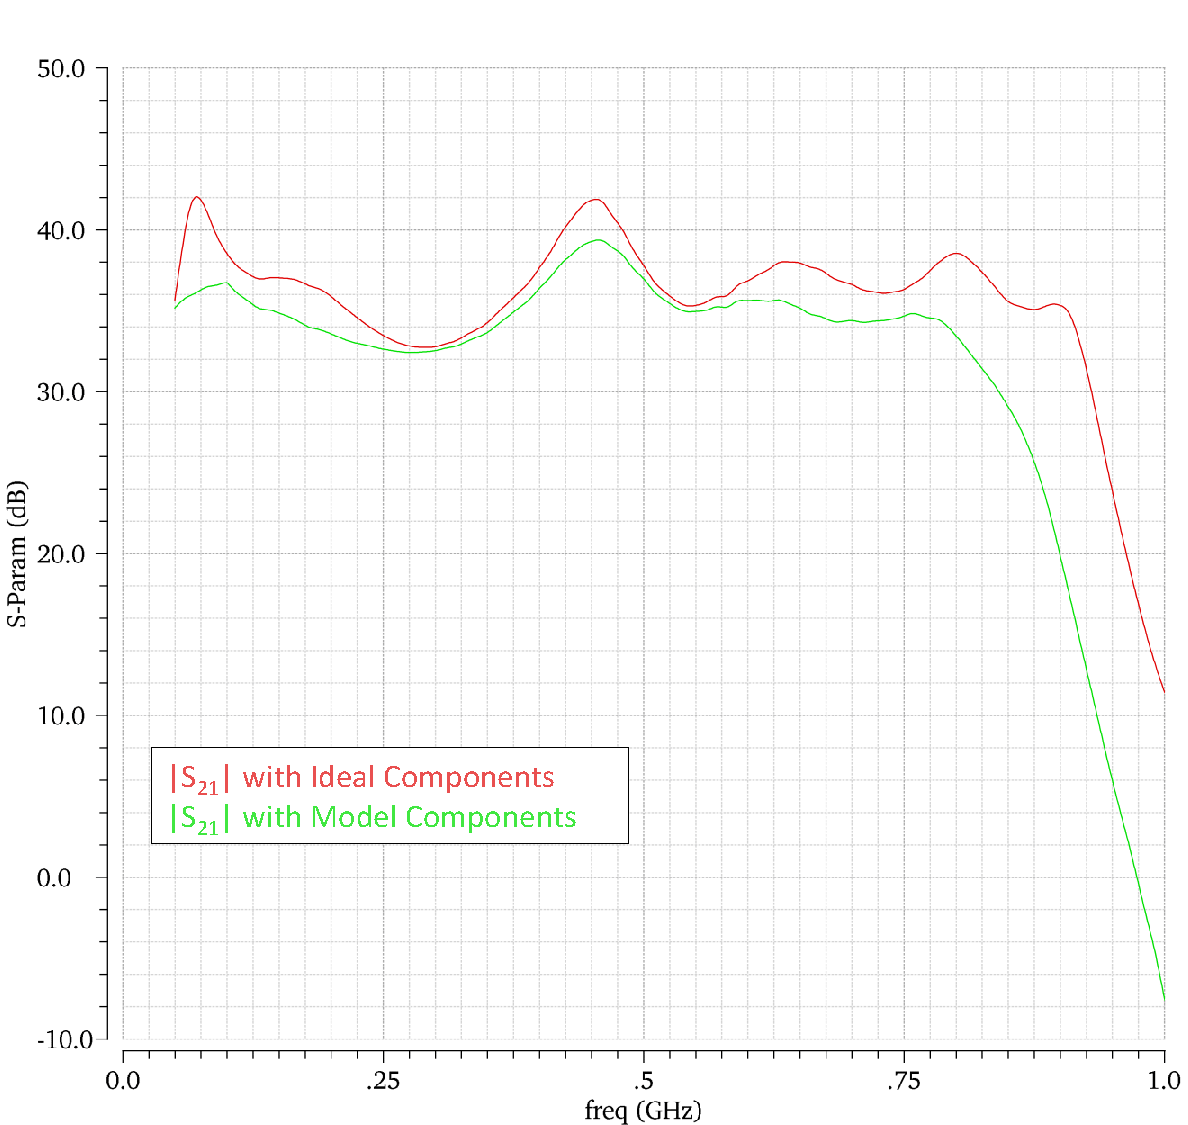
\includegraphics[width=0.7\linewidth]{figs/matching/spectre_simulation_results}   
    \caption{Simulated gain for the SpectreRF system in Figure~\ref{fig_spectre_uhf_circuit}.}
\label{fig_spectre_uhf_results}
\end{figure}
	

	In order to validate the final implemented design and understand how manufacturing process variation might effect the output frequency response of multiple RF chains in a \ac{MU-MIMO} system, we built a Python-based batch interface to the \ac{WURC}'s serial UART in order to sweep transmit frequencies while simultaneously controlling a bench-top vector signal analyzer to measure the output power \cite{guerra2012wurc_cal}.
	We implemented a digital frequency synthesizer within the digital baseband reference design for \ac{WURC} in order to generate a constant-power \ac{CW} complex sinusoid for ease of measurement.

% Output WURC power across multiple boards
\begin{figure}[ht!]
\centering
  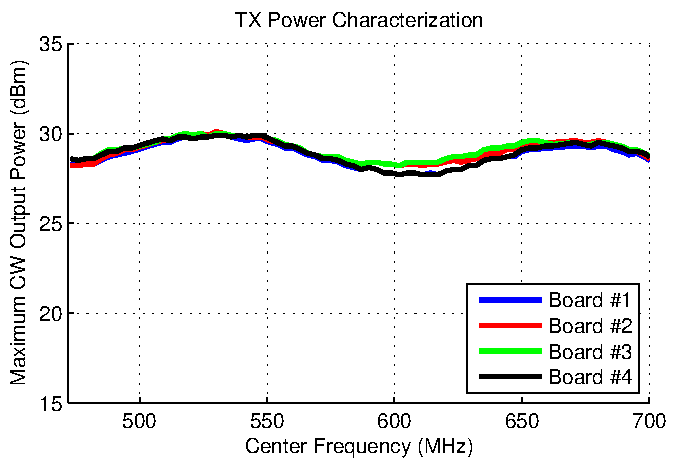
\includegraphics[width=0.8\linewidth]{figs/wurc/wurc_tx_power_plot}
    \caption{Maximum linear \ac{CW} output power as a function of center frequency for multiple \ac{WURC} units.}
		\label{fig_wurc_linear_power}
\end{figure}

	The process variation plot in Figure~\ref{fig_wurc_linear_power} was generated by increasing the output transmit gain of each \ac{WURC} at each center frequency until its output power amplifier began to saturate (\emph{i.e.} the last tested value where a 1:1 input:output gain relationship still held).
This is the delivered output power of \ac{WURC} just before the 1~dB compression point of the RF chain.
Notably, the process variation across different boards is less than 1~dB, with passband ripple on the order of 2.5~dB.
This means that multiple RF chains will maintain similar output power across the entire UHF frequency range, vastly simplifying system planning and gain control processes.

\subsection{Conclusion and Discussion}

	While this is a lengthy discussion, we believe there is valuable insight in presenting the step-by-step design and optimization of the \ac{WURC} broadband power transfer network as this work took years to develop and refine through various steps of manufacture and has application beyond this single design.
	We have attempted to not only provide enough information to replicate these design steps, but also provide motivation as to why certain decisions were made.
	%In addition, the real-frequency design code is also available open-source with permission from Yarman \cite{a_github_repo}.

	The final implemented UHF-band analog RF chain for \ac{WURC} provides up to 30~dB of static transmit gain, and up to 61~dB of dynamic receive gain, which combined with its on-board static \ac{LNA} can provide up to 83~dB of receive gain for improved sensitivity, although noise figure considerations generally limit this application to 72~dBm of dynamic receive gain.

 While we present a direct comparison of different manufactured \ac{WURC} boards demonstrating their consistent performance in Figure~\ref{fig_wurc_linear_power}, today we have manufactured dozens of \ac{WURC} boards with consistent results and also hundreds of related radio modules that utilize this same broadband power transfer design techniques for a wide range of operational frequencies and components.
	
	In conclusion, we find that the original real frequency circuit synthesis technique doesn't capture physical implementation tradeoffs well and made several changes to the design technique in order to improve the chance for success of the physical circuit realization:

\begin{enumerate}
	\item Instead of cascading multiple amplifier blocks in a series of dependent optimizations as proposed by Yarman \cite{yarman1982simplified}, we instead match the input and output of each amplifier to 50~$\Omega$ as proposed in our Section~\ref{sec_srft_problem_statement} problem statement and cascade them into each other. This allows us to decouple the design and optimization of the broadband matching network for each component and avoid the need to accurately model the microstrip feeds between amplification stages so long as they are placed in a nominal 50~$\Omega$ system.
	
	\item We utilize a simulation environment that either explicitly models package, pad, and trace parasitics or utilized empirical S-parameter models for linear system analysis. These types of tools are able to model and highlight implementation issues that are not apparent from the ideal circuits synthesized by the real frequency technique. Specifically, we present an example using Cadence Virtuoso SpectreRF in this thesis and currently use Keysight Genesys for this purpose.
	
	\item Finally, we add an additional hand-optimization step that utilizes linear analysis tools like SpectreRF or Genesys to adjust real component values based on their packages and parasitic properties in order to tune the physical circuit so that it approaches the ideal synthesized behavior. Today this is done in a greedy method whereby each component is individually hand-optimized, however the roadmap for future work to automate this with a discrete non-linear optimization algorithm using a library of empirical parts data is clear.
\end{enumerate}